\chapter{Classification \label{chapter:classification}}
One of the earliest application of artificial intelligence is 
\href{https://en.wikipedia.org/wiki/Statistical_classification}{classification}.  A good
example of classification is \href{https://en.wikipedia.org/wiki/Anti-spam_techniques#Detecting_spam}{spam detection}.
A system for spam detection classifies an email as either spam or not spam, where ``not spam'' is often
abbreviated as ``ham''.  To do so, it first
computes various \blue{features} \index{feature} of the email and then uses these features to determine whether
the email is likely to be spam.  For example, a possible feature would be the number of occurrences of the word
``\texttt{pharmacy}'' in the text of the email.

Another famous example of classification is \blue{character recognition}.  In character recognition, the
input is an image depicting a character.  This image is usually coded as a vector of grey values.  The task is
then to recognize the letter shown.  While spam detection is a \blue{binary} classification problem, character
recognition is a \blue{multi-class} classification problem, since there are 26 different characters.

\section{Introduction}
Formally, the \blue{classification problem} \index{classification problem} 
in machine learning can be stated as follows:  We are given a
set of objects $S := \{ o_1, \cdots, o_n \}$ and a set of classes $C := \{ c_1, \cdots, c_k \}$.  Furthermore, there exists a function 
\\[0.2cm]
\hspace*{1.3cm}
$\mathtt{classify}: S \rightarrow C$
\\[0.2cm]
that assigns a class $\texttt{classify}(o)$ to every object $o \in S$.  The set $S$ is called the \blue{sample space}.
In the example of spam detection, the sample space $S$ is the set of all emails that we might receive, i.e.~$S$
is the set of all strings, while the set of classes $C$ is given as
\\[0.2cm]
\hspace*{1.3cm}
$C = \{ \mathtt{spam}, \mathtt{ham} \}$.
\\[0.2cm]
Our goal is to compute the function \texttt{classify}.  In order to do this, we use an approach known as
\href{https://en.wikipedia.org/wiki/Supervised_learning}{supervised learning}:  We take a subset $S_\textsl{train} \subseteq S$ of
emails where we already know whether the emails are spam or not.  This set $S_\textsl{train}$ is called the
\blue{training set}. \index{training set}
Next, we define a set of $D$ \blue{features} for every $o \in S$.  These features have to be \blue{computable},
i.e.~we must have a function
\\[0.2cm]
\hspace*{1.3cm}
$\mathtt{feature}: S \times \{ 1, \cdots, D \} \rightarrow \mathbb{R}$ 
\\[0.2cm]
such that $\mathtt{feature}(o, j)$ computes the $j$-th feature and we have to be able to implement
this function with reasonable efficiency.  In general, the values of the features are real values.
However, there are cases where these values are just 
Booleans.  If
\\[0.2cm]
\hspace*{1.3cm}
$\texttt{feature}(o, j) \in \mathbb{B}$ \quad for all $o \in S$,
\\[0.2cm]
then the $j$-th feature is called a \blue{binary feature}.  \index{binary feature}
If we encode $\mathtt{false}$ as $-1$ and $\mathtt{true}$ as
$+1$, then the set of Boolean values $\mathbb{B}$ can be considered a subset of $\mathbb{R}$ and hence Boolean features can be considered
as real numbers.  For example, in the case of spam detection, the first feature
could be the occurrence of the string ``\texttt{pharmacy}''.  In this case, we would have
\\[0.2cm]
\hspace*{1.3cm}
$\texttt{feature}(o, 1) := \left\{
\begin{array}{ll}
  +1 & \mbox{if \ $\texttt{pharmacy}     \in o$,}      \\
  -1 & \mbox{if \ $\texttt{pharmacy} \not\in o$,}  
\end{array}\right.
$
\\[0.2cm]
i.e.~the first feature would be to check whether the email $o$ contains the string ``\texttt{pharmacy}''.  
If we want to be more precise, we can instead define the first feature as
\\[0.2cm]
\hspace*{1.3cm}
$\texttt{feature}(o, 1) := \mathtt{count}(\texttt{"pharmacy"}, o)$,
\\[0.2cm]
i.e.~we would count the number of occurrences of the string ``\texttt{pharmacy}'' in our email $o$.   
As the value of
\\[0.2cm]
\hspace*{1.3cm}
 $\mathtt{count}(\texttt{"pharmacy"}, o)$ 
\\[0.2cm]
is always a natural number, in this case the first feature would be a
 \blue{discrete} feature.  However, we can be even more precise: Instead of just counting the number of occurrences of
 ``\texttt{pharmacy}'' we can compute its \blue{frequency}.  \index{frequency}
 After all, there is a difference whether the
 string ``\texttt{pharmacy}'' occurs once in an email  containing but a hundred characters or whether is occurs
 once in an email with a length of several thousand  characters.  To this end, we would then define the first feature as
\\[0.2cm]
\hspace*{1.3cm}
$\ds \texttt{feature}(o, 1) := \frac{\mathtt{count}(\texttt{"pharmacy"}, o)}{\mathtt{len}(o)}$, 
\\[0.2cm]
where $\mathtt{len}(o)$ defines the number of characters in the string $o$.  In this case, the first feature would be a
\blue{continuous} feature and as this is the most general case, unless stated otherwise, we deal with the continuous
case. 

Having defined the features, we next need a \blue{model} of the function \texttt{classify} that tries to approximate the
function \texttt{classify} via the features.  This model is given by a function
\\[0.2cm]
\hspace*{1.3cm}
$\mathtt{model}: \mathbb{R}^D \rightarrow C$
\\[0.2cm]
such that
\\[0.2cm]
\hspace*{1.3cm}
$\mathtt{model}\bigl(\mathtt{feature}(o,1), \cdots, \mathtt{feature}(o,D)\bigr) \approx \mathtt{classify}(o)$.
\\[0.2cm]
Using the function \texttt{model}, we can then approximate the function classify using a function \texttt{guess} that is
defined as
\\[0.2cm]
\hspace*{1.3cm}
$\mathtt{guess}(o) := \mathtt{model}\bigl(\mathtt{feature}(o,1), \cdots, \mathtt{feature}(o,D)\bigr)$
\\[0.2cm]
Most of the time, the function \texttt{guess} will only \blue{approximate} the function \texttt{classify}, i.e.~we will have
\\[0.2cm]
\hspace*{1.3cm}
$\mathtt{guess}(o) = \mathtt{classify}(o)$
\\[0.2cm]
for most objects of $o \in S$ but not for all of them.  The \blue{accuracy} \index{accuracy} of our model is
defined as the fraction of those objects that are classified correctly, i.e.~
\\[0.2cm]
\hspace*{1.3cm}
$\ds \mathtt{accuracy} := \frac{\;\mathtt{card}\bigl( \{ o \in S \mid \mathtt{guess}(o) = \mathtt{classify}(o)\}\bigr)\;}{\mathtt{card}(S)}$.
\\[0.2cm]
To keep matters simple, we will assume that the sample space is finite.

The function $\mathtt{model}$ is usually determined by a set of \blue{parameters} or \blue{weights} $\mathbf{w}$. In
this case, we have
\\[0.2cm]
\hspace*{1.3cm}
$\mathtt{model}(\mathbf{x}) = \mathtt{model}(\mathbf{x},\,\mathbf{w})$
\\[0.2cm]
where $\mathbf{x}$ is the vector of features, while $\mathbf{w}$ is the vector of weights.  Later, when we
introduce \blue{logistic regression}, we will assume that the number of weights is one more than the number of
features.  Then, the weights specify the relative importance of the different features. Furthermore, there will
be a weight that is interpreted as a \blue{bias term}. \index{bias term}

When it comes to the choice of model, it is important to understand that, at least in practical applications,
\underline{all} models are wrong.  Nevertheless, \underline{some} models are useful.  There are two reasons for this:
\begin{enumerate}
\item We do not fully understand the function \texttt{classify} that we want to approximate by the function $\mathtt{model}$.
\item In the most general setting, the function \texttt{classify} is so complex, that even if we could compute
      it exactly, the resulting model would be much too complicated.
\end{enumerate}
The situation is similar in physics: Let us assume that we intend to model the fall of an object.  A model that is a
hundred percent accurate would have to include the following forces:
\begin{enumerate}[(a)]
\item gravitational acceleration,
\item air friction, 
\item tidal forces, i.e.~the effects that the rotation of the earth has on moving objects,
\item celestial forces, i.e.~the gravitational acceleration caused by celestial objects like the moon or the
      sun.
\item In the case of a metallic object we have to be aware of the magnetic forces
      caused by the \href{https://www.britannica.com/science/geomagnetic-field}{geomagnetic field}.
\item To be fully accurate, we might have to include corrections from relativistic physics and even quantum
      physics.   
\item As physics is not a closed subject, there might be other forces at work which we still do not know of. 
\end{enumerate}
Hence, a correct model would be so complicated that it would be unmanageable and therefore useless. 

Let us summarize our introductory discussion of machine learning in general and classification in particular.
A set $S$ of objects and a set $C$ of classes are given.  Our goal is to approximate a function
\\[0.2cm]
\hspace*{1.3cm}
$\mathtt{classify}: S \rightarrow C$
\\[0.2cm]
using certain \blue{features} \index{feature} of our objects.  The function $\mathtt{classify}$ is then approximated using a function
\texttt{model} as follows:
\\[0.2cm]
\hspace*{1.3cm}
$\mathtt{model}\bigl(\mathtt{feature}(o,1), \cdots, \mathtt{feature}(o,D), \mathbf{w}\bigr) \approx \mathtt{classify}(o)$.
\\[0.2cm]
The model depends on a vector of parameters $\mathbf{w}$.  In order to \blue{learn} these parameters, we are given a 
\blue{training set} $S_\textsl{train}$ that is a subset of $S$.  As we are dealing with \blue{supervised learning},
\index{supervised learning} the function 
$\mathtt{classify}$ is known for all objects $o \in S_\textsl{train}$.   Our goal is to determine the parameters $\mathbf{w}$ such that the
number of mistakes we make on the training set is minimized.  

\subsection{Notation}
We conclude this introductory section by fixing some notation.  Let us assume that the objects $o \in S_\textsl{train}$
are numbered 
from $1$ to $N$, while the features are numbered from $1$ to $D$.  Then we define
\begin{enumerate}
\item $\textbf{x}_i := \langle\mathtt{feature}(o_i, 1), \cdots, \mathtt{feature}(o_i, D)\rangle^\top$ \quad for all $i \in \{1, \cdots, N\}$.
  
      i.e.~$\mathbf{x}_i$ is a $D$-dimensional column vector that collects the features of the $i$-th training object.
\item $x_{i,j} := \mathtt{feature}(o_i, j)$ \quad for all $i \in \{1, \cdots, N\}$ and $j \in \{1, \cdots, D\}$.

      i.e.~$x_{i,j}$ is the $j$-th feature of the $i$-th object.  The numbers $x_i{i,j}$ are combined into the
      feature matrix $X$, \index{feature matrix} i.e.~we have
      \\[0.2cm]
      \hspace*{1.3cm}
      $X=(x_{i,j})_{i\in\{1,\cdots,N\} \atop j \in \{1,\cdots,D\}.}$ 
\item $y_i := \mathtt{classify}(o_i)$ \quad for all $i \in \{1, \cdots, N\}$

      i.e.~$y_i$ is the class of the $i$-th object.  These number are collected into the $N$-dimensional column vector $\mathbf{y}$.
\end{enumerate}

\subsection{Applications of Classification}
Besides spam detection, there are many other classification problems that can be solved using machine learning.  To give
just one more example, imagine a general practitioner that receives a patient and examines her symptoms.  In this case,
the symptoms can be seen as the features of the patient.  For example, these features could be
\begin{enumerate}[(a)]
\item body temperature,
\item blood pressure,
\item heart rate,
\item body weight,
\item breathing difficulties,
\item age,
\end{enumerate}
to name but a few of the possible features.  Based on these symptoms, the general practitioner would then decide on an
illness, i.e.~the set of classes for the classification problem would be
\\[0.2cm]
\hspace*{1.3cm}
$\{ \mathtt{commonCold}, \mathtt{pneumonia}, \mathtt{asthma}, \mathtt{flu}, \texttt{Covid-19}, \cdots, \mathtt{unknown} \}$.
\\[0.2cm]
Hence, the task of disease diagnosis is a classification problem.  This was one of the earliest problems that
was tackled by artificial intelligence.  As of today, 
\href{https://en.wikipedia.org/wiki/Computer-aided_diagnosis}{computer-aided diagnosis} and 
\href{https://en.wikipedia.org/wiki/Clinical_decision_support_system}{clinical decision support systems}
have been used for more than 40 years in many hospitals.  Today, there are a number of diseases that can be
diagnosed more accurately by a computer than by a specialist.  One such example is the
\href{http://www.ultromics.com}{diagnosis of heart disease}.  Other applications of classification are the following:
\begin{enumerate}[(a)]
\item image recognition,
\item speech recognition,
\item credit card fraud detection,
\item credit approval.
\end{enumerate}

\section{Digression: The Method of Gradient Ascent \label{section:gradient-ascent}}
\index{gradient ascent}
In machine learning, it is often the case that we have to find either the \blue{maximum} or the \blue{minimum}
of a function 
\\[0.2cm]
\hspace*{1.3cm}
$f: \mathbb{R}^n \rightarrow \mathbb{R}$.
\\[0.2cm]
For example, when we discuss \blue{logistic regression} in the next section, we will have to find the maximum
of the \blue{likelihood} function.  To proceed, let us introduce the \blue{$\arg\max$} function.
\index{arg max function} The idea is that
\\[0.2cm]
\hspace*{1.3cm}
$\mathbf{\widehat{x}} = \arg\max\limits_{\mathbf{x}\in \mathbb{R}^n} f$
\\[0.2cm]
is that value of $\mathbf{x} \in \mathbb{R}^n$ that maximizes $ f(\mathbf{x})$.  Formally, we have
\\[0.2cm]
\hspace*{1.3cm}
$\forall \mathbf{x} \in \mathbb{R}^n : f(\mathbf{x}) \leq f\Bigl(\arg\max\limits_{\mathbf{x}\in \mathbb{R}^n} f\Bigr)$.
\\[0.2cm]
Of course, the expression $\arg\max\limits_{\mathbf{x}\in \mathbb{R}^n} f$ is only defined when the maximum of
$f$ is unique.  If the function $f$ is differentiable, we know that a necessary condition for a vector
$\mathbf{\widehat{x}} \in \mathbb{R}^n$ to satisfy
\\[0.2cm]
\hspace*{1.3cm}
$\mathbf{\widehat{x}} = \arg\max\limits_{\mathbf{x}\in \mathbb{R}^n} f$ \quad is that we must have \quad $\nabla f(\mathbf{\widehat{x}}) = \mathbf{0}$,
\\[0.2cm]
i.e.~the \href{https://en.wikipedia.org/wiki/Gradient}{gradient} of $f$, which we will write as $\nabla f$,
vanishes at the maximum $\mathbf{\widehat{x}}$.

\begin{figure}[!th]
\centering
\hspace*{-1.3cm}
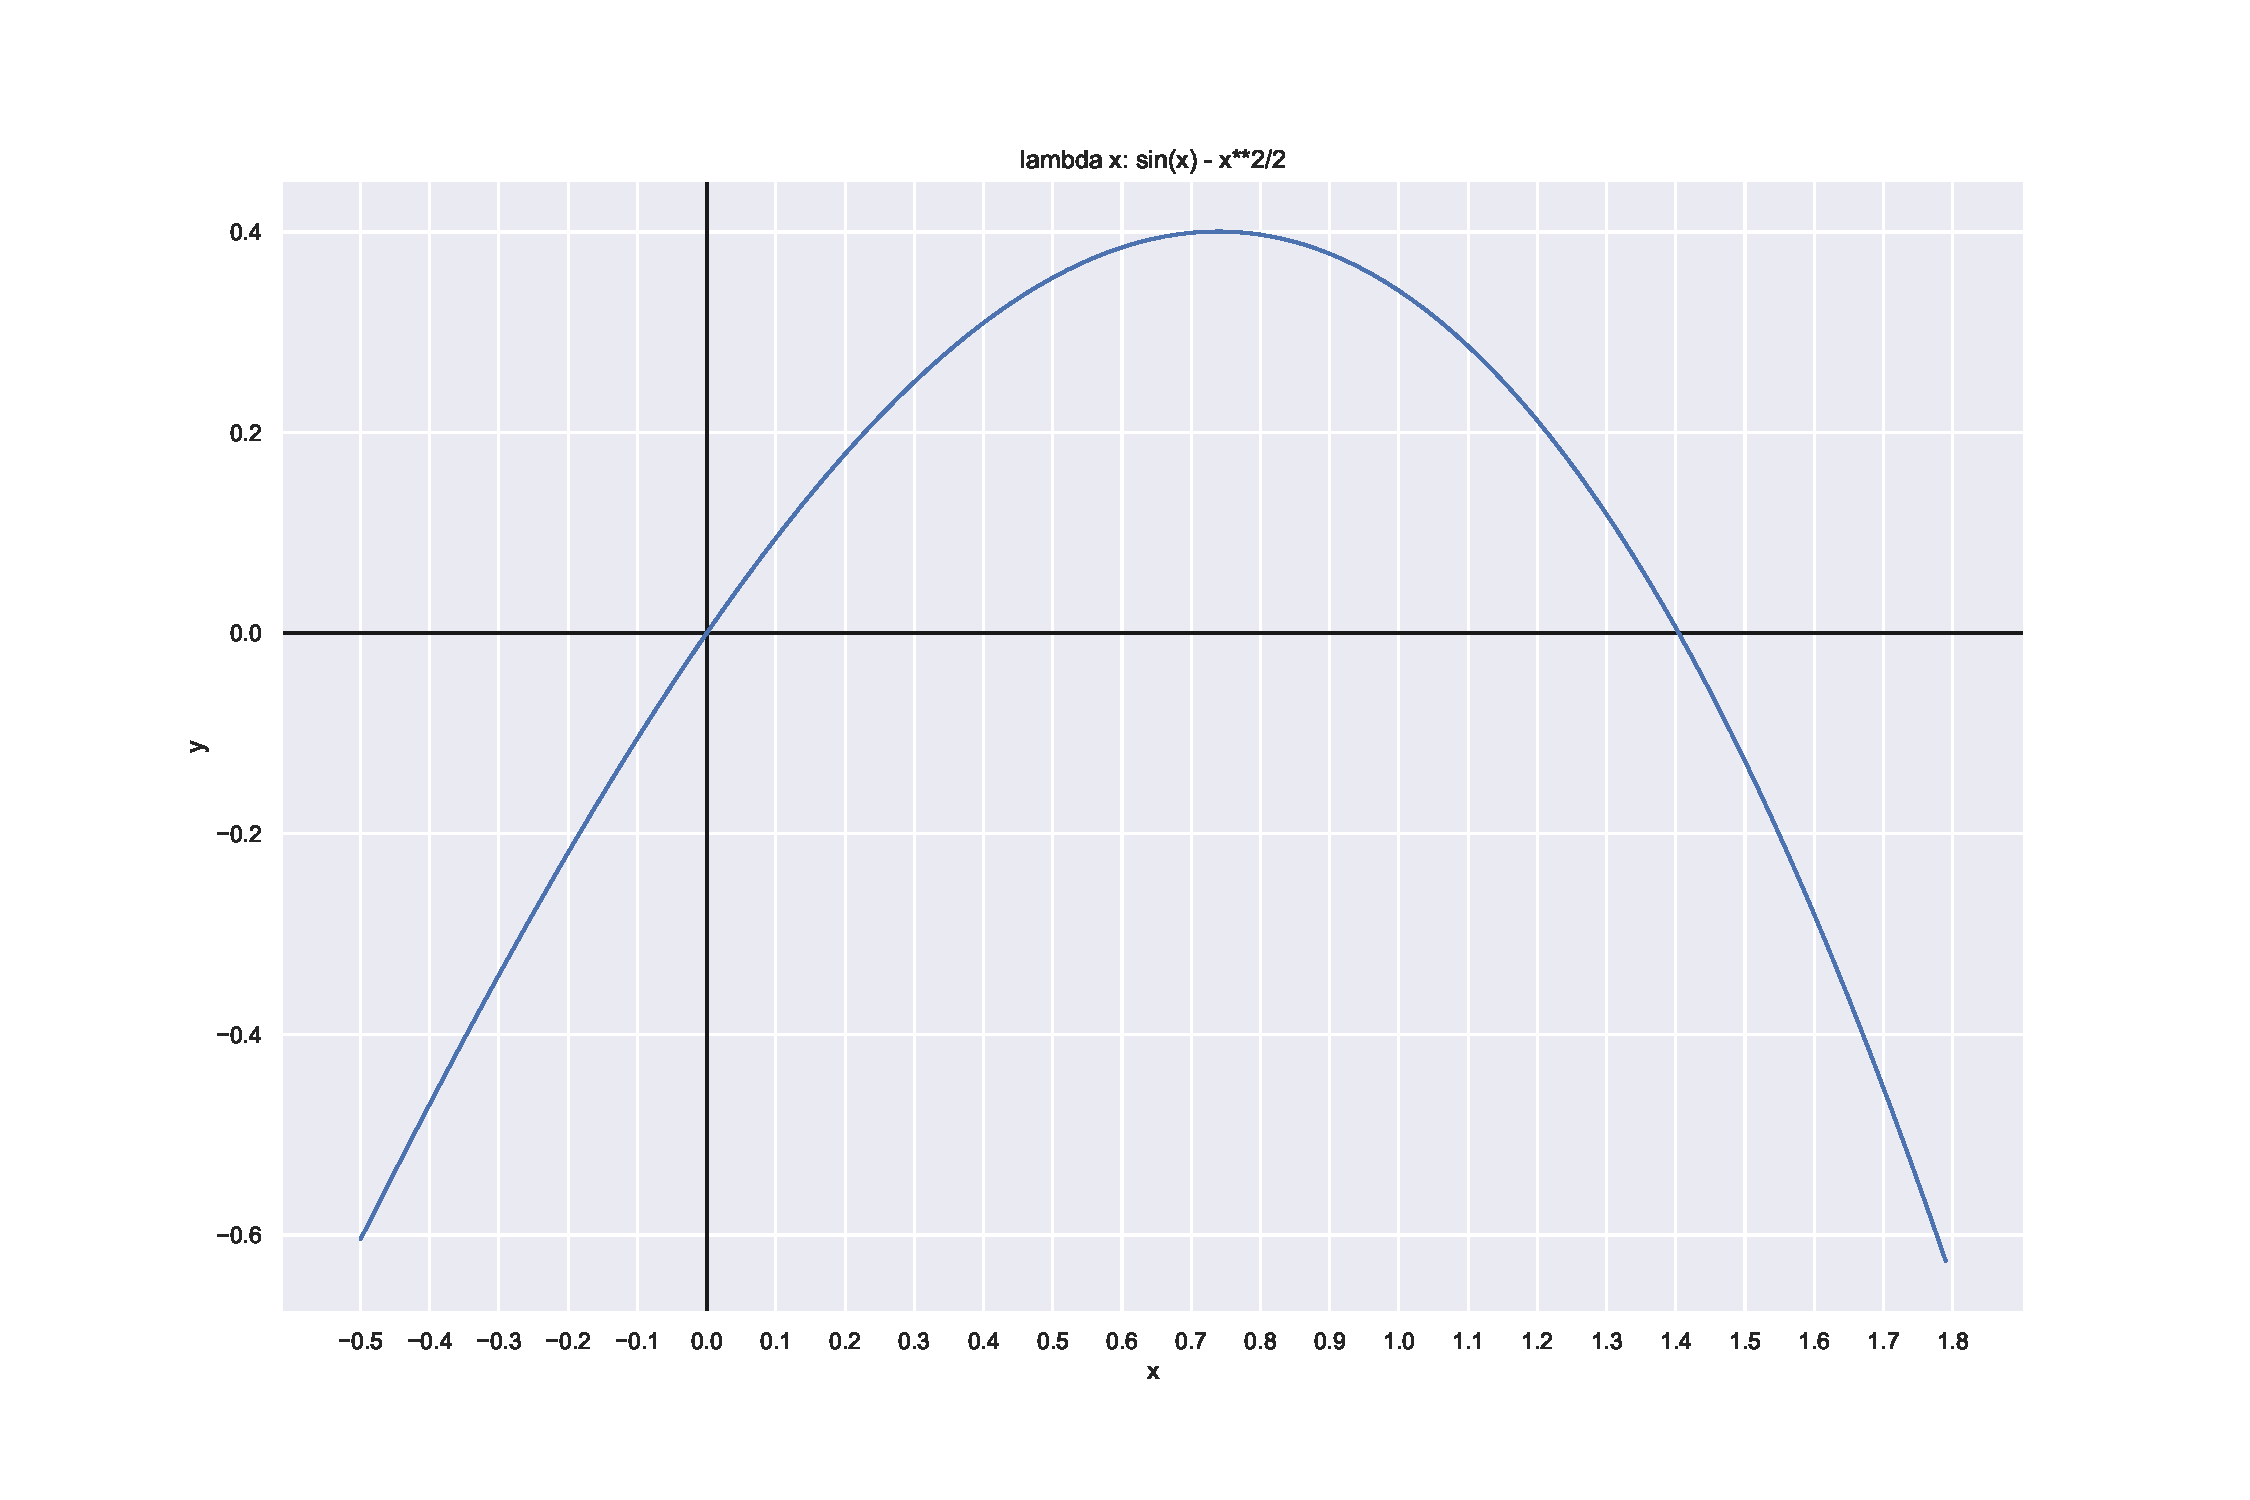
\epsfig{file=Figures/sin-minus-square.pdf, scale=0.5}
\vspace*{-0.3cm}
\caption{The function $x \mapsto \sin(x) - \frac{1}{2} \cdot x^2$.}
\label{fig:sin-minus-square.pdf}
\end{figure}

\noindent
Remember that the gradient of the function $f$ is defined as the column vector
\\[0.2cm]
\hspace*{1.3cm}
$\ds \nabla f :=
    \left\langle \frac{\partial f}{\partial\, x_1}, \cdots, \frac{\partial f}{\partial\, x_n} \right\rangle^\top
$.
\vspace*{0.2cm}

\noindent
Unfortunately, in many cases the equation 
\\[0.2cm]
\hspace*{1.3cm}
$\nabla f(\mathbf{\widehat{x}}) = \mathbf{0}$
\\[0.2cm]
cannot be solved in \href{https://en.wikipedia.org/wiki/Closed-form_expression}{closed terms}.  This is already
true in the one-dimensional case, i.e.~if $n=1$.  For example, consider 
the function $f:\mathbb{R} \rightarrow \mathbb{R}$ that is defined as
\\[0.2cm]
\hspace*{1.3cm}
$\ds f(x) := \sin(x) - \frac{1}{2} \cdot x^2$.
\\[0.2cm]
This function is shown in Figure \ref{fig:sin-minus-square.pdf} on page \pageref{fig:sin-minus-square.pdf}.
From the graph of the function it is obvious that this function has a maximum somewhere between $0.6$ and
$0.8$.  In order to compute this maximum, we can compute the derivative of $f$.   This derivative is given as 
\\[0.2cm]
\hspace*{1.3cm}
$f'(x) = \cos(x) - x$
\\[0.2cm]
As it happens, the equation $\cos(x) - x = 0$ does not seem to have a solution in 
\href{https://en.wikipedia.org/wiki/Closed-form_expression}{closed form}.  Hence, we can only approximate
the solution numerically via a sequence of numbers $(x_n\bigr)_{n\in\mathbb{N}}$ such that the limit
$\ds \lim\limits_{n\rightarrow\infty} x_n$
exists and is a solution of the equation $\cos(x) - x = 0$, i.e.~we want to have
\\[0.2cm]
\hspace*{1.3cm}
$\ds \cos\Bigl(\lim\limits_{n\rightarrow\infty} x_n\Bigr) = \lim\limits_{n\rightarrow\infty} x_n$.
\\[0.2cm]
The method of \href{https://en.wikipedia.org/wiki/Gradient_descent}{gradient ascent} is a numerical
method that can be used to find the maximum of a function 
\\[0.2cm]
\hspace*{1.3cm}
$f: \mathbb{R}^n \rightarrow \mathbb{R}$
\\[0.2cm]
numerically.  The basic idea is to take a vector $\mathbf{x}_0 \in \mathbb{R}^n$ as the start value and define a sequence of
vectors $\bigl(\mathbf{x}_n\bigr)_{n\in\mathbb{N}}$ such that we have
\\[0.2cm]
\hspace*{1.3cm}
$f(\mathbf{x}_{n+1}) \geq f(\mathbf{x}_{n})$ \quad for all $n\in\mathbb{N}$.
\\[0.2cm]
Hopefully, this sequence will converge against $\widehat{\mathbf{x}} = \arg\max\limits_{\mathbf{x}\in \mathbb{R}^n}f$.
If we do not really know where to start our search, we define $\mathbf{x}_0 := \mathbf{0}$.  In order to
compute $\mathbf{x}_{n+1}$ given $\mathbf{x}_{n}$, the idea is to move from $\mathbf{x}_n$ in that direction
where we have the biggest change in the values of $f$.   This direction happens to be the gradient of $f$ at $\mathbf{x}_n$.
Therefore, the definition of $\mathbf{x}_{n+1}$ is given as follows:
\\[0.2cm]
\hspace*{1.3cm}
$\mathbf{x}_{n+1} := \mathbf{x}_n + \alpha \cdot \nabla f(\mathbf{x}_n)$ \quad for all $n \in \mathbb{N}_0$.
\\[0.2cm]
Here, $\alpha$ is called the \blue{step size} and is also known as the \blue{learning rate}.  It determines by how
much we move in the direction of the gradient.  In practise, it is best to adapt the step size dynamically
during the iterations.  Figure \ref{fig:gradient-ascent.py} on page \pageref{fig:gradient-ascent.py} shows
how this is done. 
The function \texttt{findMaximum} takes four arguments:
\begin{enumerate}
\item $\texttt{f}$ is the function that is to be maximized.  It is assumed that \texttt{f} takes a vector
      $\texttt{x}\in \mathbb{R}^n$ as its input and that it returns a real number.  Note that $n$ might be
      $1$.  In that case the input to $f$ is a real number.
\item $\texttt{gradF}$ is the gradient of \texttt{f}.  It takes a vector
      $\texttt{x}\in \mathbb{R}^n$ as its input and returns the vector $\nabla \mathtt{f}(\mathtt{x})$.
\item $\texttt{start}$ is a vector from $\mathbb{R}^n$ that is used as the value of $\mathbf{x}_0$.  In
      practice, we will often use $\mathbf{0} \in \mathbb{R}^n$ as the start vector.
\item $\texttt{eps}$ is the precision that we need for the maximum.  We will have to say more on how \texttt{eps}
      is related to the precision later.  As we are using double precision floating point arithmetic, 
      it won't make sense to use a value for \texttt{eps} that is smaller than $10^{-15}$.
\end{enumerate}
Next, let us discuss the implementation of gradient ascent.
\begin{enumerate}
\item \texttt{x} is initialized with the parameter \texttt{start}.  Hence, \texttt{start} is really the same as
      $\mathbf{x}_0$. 
\item \texttt{fx} is the value $\texttt{f}(\texttt{x})$.
\item \texttt{alpha} is the \blue{learning rate}.  We initialize \texttt{alpha} as $1.0$.  The learning rate
      will be adapted dynamically. 
\item The body of the \texttt{while} loop starting in line 6 executes one iteration of gradient ascent.
\item In each iteration, we store the values of $\mathbf{x}_n$ and $f(\mathbf{x}_n)$ in the variables
      \texttt{xOld} and \texttt{fOld}.  This is needed since we need to ensure that the values of
      $f(\mathbf{x}_n)$ are increasing.  If this value of $f(\mathbf{x}_{n+1})$ is not bigger that
      $f(\mathbf{x}_n)$ we revert to the old values.
\item Next, we compute $\mathbf{x}_{n+1}$ in line 8 using the formula
      \\[0.2cm]
      \hspace*{1.3cm}
      $\mathbf{x}_{n+1} := \mathbf{x}_n + \alpha \cdot \nabla f(\mathbf{x}_n)$.
\item The corresponding value $f(\mathbf{x}_{n+1})$ is computed in line 9.
\item If we are unlucky, $f(\mathbf{x}_{n+1})$ is smaller than $f(\mathbf{x}_{n})$ instead of bigger.  This might happen if the learning
      rate $\alpha$ is too large.  Hence, in this case we decrease the value of $\alpha$, discard 
      both $\mathbf{x}_{n+1}$ and $f(\mathbf{x}_{n+1})$ and start over again via the \texttt{continue}
      statement in line 13.
\item Otherwise, if  $f(\mathbf{x}_{n+1})$ is indeed bigger than $f(\mathbf{x}_{n})$, the vector
  $\mathbf{x}_{n+1}$ is a better approximation of the maximum than the vector $\mathbf{x}_n$.  
      In this case, in order to increase the speed of the convergence of our algorithm we will then increase the learning rate
      $\alpha$ by $20\%$.    
\item The idea of our implementation is to stop the iteration when the relative difference  of 
      $f(\mathbf{x}_{n+1})$ and $f(\mathbf{x}_{n})$ is less than $\varepsilon$ or, to be more precise, if
      \\[0.2cm]
      \hspace*{1.3cm}
      $f(\mathbf{x}_{n+1}) < f(\mathbf{x}_{n}) \cdot (1 + \varepsilon)$.
      \\[0.2cm]
      As the sequence $\bigl(f(\mathbf{x}_n\bigr)_{n\in\mathbb{N}}$ will be monotonically
      increasing, i.e.~we have
      \\[0.2cm]
      \hspace*{1.3cm}
      $f(\mathbf{x}_{n+1}) \geq f(\mathbf{x}_{n})$ \quad for all $n\in\mathbb{N}$,
      \\[0.2cm]
      the condition given above is sufficient.  Now, if the increment of  $f(\mathbf{x}_{n+1})$ is less than $f(\mathbf{x}_{n}) \cdot (1 + \varepsilon)$ 
      we assume that we have reached the maximum with the required precision.  In this case we return both the
      value of \texttt{x} and the corresponding function value $f(\mathtt{x})$.
\end{enumerate}

\begin{figure}[!ht]
\centering
\begin{minted}[ frame         = lines, 
                framesep      = 0.3cm, 
                firstnumber   = 1,
                bgcolor       = sepia,
                mathescape,
                numbers       = left,
                numbersep     = -0.2cm,
                xleftmargin   = 0.8cm,
                xrightmargin  = 0.8cm,
              ]{python3}
    def findMaximum(f, gradF, start, eps):
        x     = start
        fx    = f(x)
        alpha = 1.0
        cnt   = 1  # number of iterations
        while True:
            xOld, fOld = x, fx
            x  += alpha * gradF(x)
            fx  = f(x)
            if fx <= fOld:   
                alpha *= 0.5
                x, fx = xOld, fOld
                continue
            else:
                alpha *= 1.2
            if abs(fx - fOld) <= abs(fx) * eps:
                return x, fx
            cnt += 1                  
\end{minted}

\caption{The gradient ascent algorithm.}
\label{fig:gradient-ascent.py}
\end{figure}
\FloatBarrier

The implementation of gradient ascent given above is not the most sophisticated variant of this algorithm.
Furthermore, there are algorithms that are more powerful than gradient ascent.  The first of these methods is the
\href{https://en.wikipedia.org/wiki/Conjugate_gradient_method}{conjugate gradient method}.  A
refinement of this method is the
\href{https://en.wikipedia.org/wiki/Broyden-Fletcher-Goldfarb-Shanno_algorithm}{BFGS-algorithm} that
has been invented by Broyden, Fletcher, Goldfarb, and Shanno.  Unfortunately, we do not have the
time to discuss these algorithms.
However, our implementation of gradient ascent is sufficient for our applications and as this is not a course on numerical
analysis but rather on artificial intelligence we will not delve deeper into this topic but, instead, we refer
readers interested in more efficient algorithms to the literature \cite{snyman:2005}.  If you ever need to find
the maximum of a function numerically, you should try to use a predefined library routine that implements a
state of the art algorithm.  For example, in \href{https://www.python.org}{Python} the method
\href{https://docs.scipy.org/doc/scipy/reference/generated/scipy.optimize.minimize.html#scipy.optimize.minimize}{minimize}
from the package \texttt{scipy.optimize} offers various algorithms for minimization.

\section{Logistic Regression}
\index{logistic regression}
If we have a model such that 
\\[0.2cm]
\hspace*{1.3cm}
$\mathtt{model}(\mathbf{x}, \mathbf{w}) \approx \mathtt{classify}(\mathbf{x})$
\\[0.2cm]
holds, then we want to choose the weight vector $\mathbf{w}$ in a way such that the accuracy 
\\[0.2cm]
\hspace*{1.3cm}
$\ds \mathtt{accuracy}(\mathbf{w}) := 
\frac{\;\mathtt{card}\bigl(\bigl\{ \mathbf{o} \in S \bigm| \mathtt{model}(\mathtt{feature}\bigl(\mathbf{o}),\mathbf{w}\bigr) = \mathtt{classify}(\mathbf{o})\bigr\}\bigr)\;}{\mathtt{card}(S)}$
\\[0.2cm]
is maximized.  However, there is a snag:  The accuracy is not a smooth function of the weight vector
$\mathbf{w}$.  It can't be a smooth function because the number of errors of our model is a natural number and not a real number
that could change smoothly when the weight vector $\mathbf{w}$ is changed.  Hence, the accuracy is not differentiable as a function
of the weight vector.  The way to proceed is to work with \blue{probabilities} instead.  Instead of assigning a
class to an object $\mathbf{o}$ we rather assign a \blue{probability} $p$ to the object $\mathbf{o}$ that measures how
probable it is that object $\mathbf{o}$ has a given class $c$.  Then we try to maximize this probability.  In
\href{https://en.wikipedia.org/wiki/Logistic_regression}{logistic regression} we use a linear model that is 
combined with the \blue{sigmoid function}.  Before we can discuss the details of logistic regression we need to
define this function and state some of its properties.  

\subsection{The Sigmoid Function}

\begin{figure}[!ht]
\centering
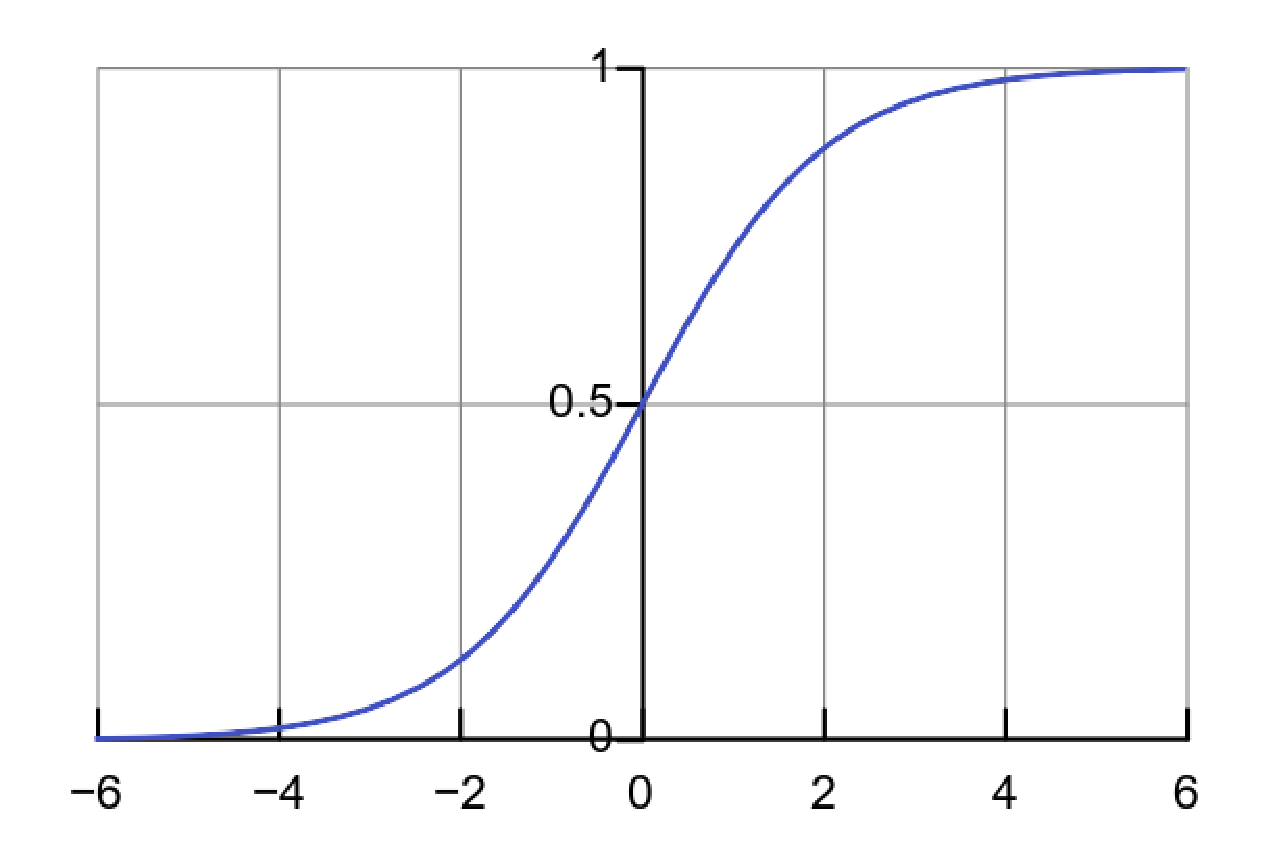
\epsfig{file=Figures/sigmoid.eps, scale=0.7}
\vspace*{-0.3cm}
\caption{The sigmoid function.}
\label{fig:sigmoid.eps}
\end{figure}
\FloatBarrier

\begin{Definition}[Sigmoid Function\label{def:sigmoid}]
  The \href{https://en.wikipedia.org/wiki/Sigmoid_function}{sigmoid function} $S: \mathbb{R} \rightarrow [0, 1]$
  \index{sigmoid function} is defined as 
\\[0.2cm]
\hspace*{1.3cm}
$\ds S(t) = \frac{1}{1 + \exp(-t)}$.  
\\[0.2cm]
Figure \ref{fig:sigmoid.eps} on page \pageref{fig:sigmoid.eps} shows the sigmoid function.
The sigmoid function is also known as the \blue{logistic function}. \index{logistic function}
\eox
\end{Definition}


\noindent
Let us note some immediate consequences of the definition of the sigmoid function.  As we have
\\[0.2cm]
\hspace*{1.3cm}
$\ds\lim\limits_{x\rightarrow-\infty} \exp(-x) = \infty$, \quad 
$\ds\lim\limits_{x\rightarrow+\infty} \exp(-x) = 0$, \quad and \quad
$\ds\lim\limits_{x\rightarrow\infty} \frac{1}{x} = 0$, 
\\[0.2cm]
the sigmoid function has the following properties:
\\[0.2cm]
\hspace*{1.3cm}
$\ds \lim_{t\rightarrow-\infty} S(t) = 0$ \quad and \quad
$\ds \lim_{t\rightarrow+\infty} S(t) = 1$.
\\[0.2cm]
As the sigmoid function is monotonically increasing, this shows that indeed 
\\[0.2cm]
\hspace*{1.3cm}
$0 \leq S(t) \leq 1$  \quad for all $t \in \mathbb{R}$.
\\[0.2cm]
Therefore, the value of the sigmoid function can be interpreted as a \blue{probability}.
Another important property of the sigmoid function is its symmetry.  Figure \ref{fig:sigmoid.eps} shows that if the
sigmoid function is shifted down by $\frac{1}{2}$, the resulting function is 
\href{https://en.wikipedia.org/wiki/Point_reflection}{centrally symmetric}, \index{centrally symmetric}
i.e.~we have
\\[0.2cm]
\hspace*{1.3cm}
$\ds S(-t) - \frac{1}{2} = -\Bigl(S(t) - \frac{1}{2}\Bigr)$.
\\[0.2cm]
Adding $\ds\frac{1}{2}$ on both sides of this equation shows that this is equivalent to the equation
\\[0.2cm]
\hspace*{1.3cm}
\colorbox{red}{\framebox{\colorbox{orange}{
$S(-t) = 1 - S(t)$,}}}
\\[0.2cm]
The proof of this fact runs as follows:
\\[0.2cm]
\hspace*{1.3cm}
$
\begin{array}{lcll}
1 - S(t) & = & \ds 1 - \frac{1}{1 + \exp(-t)}             & \mbox{(by definition of $S(t)$)}           \\[0.5cm]
         & = & \ds \frac{1 + \exp(-t) - 1}{1 + \exp(-t)}  & \mbox{(common denominator)}                \\[0.5cm]
         & = & \ds \frac{\exp(-t)}{1 + \exp(-t)}          &                                          \\[0.5cm]
         & = & \ds \frac{1}{\exp(t) + 1}                  & \mbox{(expand fraction by $\exp(t)$)}      \\[0.5cm]
         & = & \ds \frac{1}{1 + \exp(+t)}                 &                                          \\[0.5cm]
         & = & S(-t)                                      & \mbox{(by definition of $S(-t)$)}. \qquad _\Box
\end{array}
$
\\[0.2cm]
The exponential function can be expressed via the sigmoid function.  Let us start with the definition of the sigmoid
function. 
\\[0.2cm]
\hspace*{1.3cm}
$\ds S(t) = \frac{1}{1 + \exp(-t)}$
\\[0.2cm]
Multiplying this equation with the denominator yields
\\[0.2cm]
\hspace*{1.3cm}
$\ds S(t) \cdot \bigl(1 + \exp(-t)\bigr) = 1$.
\\[0.2cm]
Dividing both sides by $S(t)$ gives:
\\[0.2cm]
\hspace*{1.3cm}
$
\begin{array}{cl}
                & \ds 1 + \exp(-t) = \frac{1}{S(t)}        \\[0.5cm]
\Leftrightarrow & \ds \exp(-t) = \frac{1}{S(t)} - 1        \\[0.5cm]
\Leftrightarrow & \ds \exp(-t) = \frac{1 - S(t)}{S(t)}      
\end{array}
$
\\[0.2cm]
We highlight this formula, as we need it later
\begin{equation}
\label{eq:1}
 \colorbox{red}{\framebox{\colorbox{orange}{\mbox{$\ds\exp(-t) = \frac{1 - S(t)}{S(t)}$.}}}}
\end{equation}
If we take the reciprocal of both sides of this equation, we have
\\[0.2cm]
\hspace*{1.3cm}
$\ds \exp(t) = \frac{S(t)}{1 - S(t)}$.
\\[0.2cm]
Applying the natural logarithm on both sides of this equation yields
\\[0.2cm]
\hspace*{1.3cm}
$\ds t = \ln\left(\frac{S(t)}{1-S(t)}\right)$.
\\[0.2cm]
This shows that the inverse of the sigmoid function is given as
\\[0.2cm]
\hspace*{1.3cm}
\colorbox{red}{\framebox{\colorbox{orange}{
$\ds S^{-1} (y) = \ln\left(\frac{y}{1-y}\right)$.}}} 
\\[0.2cm]
This function is known as the \href{https://en.wikipedia.org/wiki/Logit}{logit function}.
\index{logit function}
Next, let us compute the derivative of $S(t)$, i.e.~$\ds S'(t) =\frac{\mathrm{d}S}{\mathtt{d}t}$.  We have
\\[0.2cm]
\hspace*{1.3cm}
$
\begin{array}{lcll}
 S'(t) & = & \ds -\frac{-\exp(-t)}{\bigr(1+\exp(-t)\bigr)^2}   \\[0.5cm]
       & = & \ds \exp(-t) \cdot S(t)^2                         \\[0.2cm]
       & = & \ds \frac{1-S(t)}{S(t)} \cdot S(t)^2  & \mbox{(by Equation \ref{eq:1})} \\[0.4cm]
       & = & \ds \bigl(1 - S(t)\bigr) \cdot S(t)            
\end{array}
$
\\[0.2cm]
We have shown
\begin{equation}
  \label{eq:2}
  \colorbox{red}{\framebox{\colorbox{orange}{\mbox{$\ds S'(t) = \bigl(1 - S(t)\bigr) \cdot S(t)$.}}}}
\end{equation}
We will later need the derivative of the natural logarithm of the logistic function.  We define
\\[0.2cm]
\hspace*{1.3cm}
$L(t) := \ln\bigl(S(t)\bigr)$.
\\[0.2cm]
Then we have
\\[0.2cm]
\hspace*{1.3cm}
$
\begin{array}{lcll}
  L'(t) & = & \ds \frac{S'(t)}{S(t)}                  & \mbox{(by the chain rule)} \\[0.5cm]
        & = & \ds \frac{(1 - S(t)) \cdot S(t)}{S(t)}                               \\[0.5cm]
        & = & \ds 1 - S(t)                                                         \\[0.2cm]
        & = & \ds S(-t)                               & \mbox{(by symmetry)} 
\end{array}
$
\\[0.2cm]
% If we have the function $f(t) := L(-t)$, then we see that
%\\[0.2cm]
%\hspace*{1.3cm}
% $f'(t) = -S(t)$
%\\[0.2cm]
% holds.   
As this is our most important result, we highlight it:
\\[0.2cm]
\hspace*{1.3cm}
\colorbox{red}{\framebox{\colorbox{orange}{$L'(t) = S(-t)$ \quad where \quad $L(t) := \ln\bigl(S(t)\bigr)$.}}}


\subsection{The Model of Logistic Regression}
In logistic regression we deal with \blue{binary classification}, \index{binary classification}
i.e.~we assume that we just need to decide
whether a given object is a member of a given class or not.  We use the following model to compute the \blue{probability} that an
object $o$ with features $\mathbf{x}$ will be of the given class: 
\\[0.2cm]
\hspace*{1.3cm}
$P(y=+1\;|\;\mathbf{x},\mathbf{w}) = S(\mathbf{x} \cdot \mathbf{w})$.
\\[0.2cm]
Note that $P(y=+1\;|\;\mathbf{x},\mathbf{w})$ is the \blue{conditional probability} that $o$ has the given
class, given its features $\mathbf{x}$ and the weights $\mathbf{w}$.  The expression $\mathbf{x}
\cdot \mathbf{w}$ denotes the \blue{dot product} of the vectors $\mathbf{x}$ and $\mathbf{w}$,  
i.e. we have
\\[0.2cm]
\hspace*{1.3cm}
$\mathbf{x} \cdot \mathbf{w} = \sum\limits_{i=1}^D x_i \cdot w_i$.
\\[0.2cm] 
To simplify calculations, it is assumed that $\mathbf{x}$ contains a \blue{constant feature} \index{constant feature}
that always takes the value of $1$.
Seeing this model for the first time you might think that this model is not very general and that it can only be
applied in very special circumstances.  However,  the features $x_i$ can be functions of arbitrary complexity
and hence this model is much more general than it appears on first sight.

We assume that $y$ can only take the values $+1$ or $-1$,  e.g.~in the example of spam detection $y = 1$ if the
email is spam and $y = -1$ otherwise.  Since complementary probabilities add up to $1$, we have
\\[0.2cm]
\hspace*{1.3cm}
$P(y=-1\;|\;\mathbf{x},\mathbf{w}) = 1 - P(y=+1\;|\;\mathbf{x},\mathbf{w}) 
  = 1 - S(\mathbf{x} \cdot \mathbf{w}) = S(-\mathbf{x} \cdot \mathbf{w})
$.
\\[0.2cm]
Hence, we can combine the equations for $P(y=-1\;|\;\mathbf{x},\mathbf{w})$ and $P(y=+1\;|\;\mathbf{x},\mathbf{w})$ into a
single equation
\\[0.2cm]
\hspace*{1.3cm}
\colorbox{red}{\framebox{\colorbox{orange}{$P(y\;|\;\mathbf{x},\mathbf{w}) = S\bigl(y \cdot(\mathbf{x} \cdot \mathbf{w})\bigr)$.}}}
\\[0.2cm]
Given $N$ objects $o_1, \cdots, o_n $ with feature vectors $\mathbf{x}_1, \cdots, \mathbf{x}_n$ and classes
$y_1,\cdots,y_n$, we
want to determine the weight vector $\mathbf{w}$ such that the \blue{likelihood} $\ell(\mathbf{X}, \mathbf{y})$
\index{likelihood} of all of our
observations is maximized, where $\mathbf{X}$ is the \blue{feature matrix} that is defined as
\\[0.2cm]
\hspace*{1.3cm}
$\mathbf{X} := \left(
  \begin{array}{c}
    \bigl(\mathbf{x}^{(1)}\bigr)^\top  \\
    \vdots                         \\
    \bigl(\mathbf{x}^{(m)}\bigr)^\top
  \end{array}
  \right).   
$
\\[0.2cm]
This approach is called the 
\href{https://en.wikipedia.org/wiki/Maximum_likelihood_estimation}{maximum likelihood estimation}
\index{maximum likelihood estimation} of the weights.
As we assume that the probabilities of different observations are independent, the individual
probabilities have to be multiplied to compute the overall likelihood $\ell(\mathbf{X}, \mathbf{y},\mathbf{w})$ 
of a given training set:
\\[0.2cm]
\hspace*{1.3cm}
$\ds \ell(\mathbf{X},\mathbf{y},\mathbf{w}) = \prod\limits_{i=1}^N P(y_i \;|\;\mathbf{x}_i,\mathbf{w})$.
\\[0.2cm]
Since it is easier to work with sums than with products, instead of maximizing the function
$\ell(\mathbf{X},\mathbf{y},\mathbf{w})$ we instead maximize the logarithm of
$\ell(\mathbf{X},\mathbf{y},\mathbf{w})$.  This logarithm is called the \blue{log-likelihood} \index{log-likelihood} and is defined as 
\\[0.2cm]
\hspace*{1.3cm}
$\ell\ell(\mathbf{X},\mathbf{y},\mathbf{w}) := \ln\bigl(\ell(\mathbf{X},\mathbf{y},\mathbf{w})\bigr)$. 
\\[0.2cm]
As the natural logarithm is a \href{https://en.wikipedia.org/wiki/Monotonic_function}{monotonically increasing}
function, the functions $\ell(\mathbf{X},\mathbf{y},\mathbf{w})$ and  $\ell\ell(\mathbf{X},\mathbf{y},\mathbf{w})$ take their maximum at the same value of $\mathbf{w}$.  As we have
\\[0.2cm]
\hspace*{1.3cm}
$\ln(a \cdot b) = \ln(a) + \ln(b)$,
\\[0.2cm]
the natural logarithm of the likelihood is 
\\[0.2cm]
\hspace*{1.3cm}
\colorbox{red}{\framebox{\colorbox{orange}{
$\ds \ell\ell(\mathbf{X},\mathbf{y},\mathbf{w}) = 
 \sum\limits_{i=1}^N \ln\Bigl(S\bigl(y_i \cdot(\mathbf{x}_i \cdot \mathbf{w})\bigr)\Bigr) =
 \sum\limits_{i=1}^N L\bigl(y_i \cdot(\mathbf{x}_i \cdot \mathbf{w})\bigr)
$.}}}
\\[0.2cm]
Our goal is to choose the weights $\mathbf{w}$ such that the likelihood is maximized.  Since this is the same as maximizing the log-likelihood, we
need to determine the gradient of the log-likelihood with respect to the weights $w_j$, i.e.~we need to compute
the partial derivatives
\\[0.2cm]
\hspace*{1.3cm}
$\ds \frac{\partial\quad}{\partial\, w_j}\ell\ell(\mathbf{X},\mathbf{y},\mathbf{w})$ \quad for all $j\in\{1,\cdots,D\}$.
\\[0.2cm]
In order to compute the partial derivative of $\ell\ell(\mathbf{X},\mathbf{y},\mathbf{w})$ with respect to the
coefficients $\mathbf{w}$ we need to compute the partial derivative of the dot product $\mathbf{x}_i \cdot
\mathbf{w}$ with respect to the weights $w_j$.
We define
\\[0.2cm]
\hspace*{1.3cm}
$\ds h(\mathbf{w}) := \mathbf{x}_i \cdot \mathbf{w} = \sum\limits_{k=1}^D x_{i,k} \cdot w_k$.
\\[0.2cm]
Then we have
\\[0.2cm]
\hspace*{1.3cm}
$\ds \frac{\partial\quad}{\partial\, w_j} h(\mathbf{w})
   = \frac{\partial\quad}{\partial\, w_j} \sum\limits_{k=1}^D x_{i,k} \cdot w_k
   = \sum\limits_{k=1}^D x_{i,k} \cdot \frac{\partial\quad}{\partial\, w_j} w_k
   = \sum\limits_{k=1}^D x_{i,k} \cdot \delta_{j,k} =  x_{i,j}
$.
\\[0.2cm]
Now we are ready to compute the partial derivative of $\ell\ell(\mathbf{X},\mathbf{y},\mathbf{w})$ with respect to $\mathbf{w}$:
\\[0.2cm]
\hspace*{1.3cm}
$
\begin{array}{cll}
  & \ds \frac{\partial\quad}{\partial\, w_j} \ell\ell(\mathbf{X},\mathbf{y},\mathbf{w}) \\[0.5cm]
= & \ds \frac{\partial\quad}{\partial\, w_j} 
    \sum\limits_{i=1}^N L\bigl(y_i \cdot(\mathbf{x}_i \cdot \mathbf{w})\bigr) 
    \\[0.5cm]
= & \ds\sum\limits_{i=1}^N y_i \cdot x_{i,j} \cdot  S\bigl(-y_i \cdot(\mathbf{x}_i \cdot \mathbf{w})\bigr),
  & \mbox{since} \quad \ds \frac{\mathrm{d}L(x)}{\mathrm{d}x} = S(-x).
\end{array}
$
\\[0.2cm]
Hence, the partial derivative of the log-likelihood function is given as follows:
\\[0.2cm]
\hspace*{1.3cm}
\colorbox{red}{\framebox{\colorbox{orange}{
$\ds \frac{\partial\quad}{\partial\, w_j}\ell\ell(\mathbf{X},\mathbf{y},\mathbf{w}) =
 \ds\sum\limits_{i=1}^N y_i \cdot x_{i,j} \cdot  S(-y_i \cdot \mathbf{x}_i \cdot \mathbf{w})
$}}} 
\\[0.2cm]
Next, we have to find the value of $\mathbf{w}$ such that
\\[0.2cm]
\hspace*{1.3cm}
$\ds\sum\limits_{i=1}^N y_i \cdot x_{i,j} \cdot  S(-y_i \cdot \mathbf{x}_i \cdot \mathbf{w}) = 0$
\quad for all $j \in \{1, \cdots, D\}$.
\\[0.2cm]
These are $D$ equations for the $D$ variables $w_1, \cdots, w_D$.  Due to the occurrence of the sigmoid function, these
equations are nonlinear.  We can not solve these equations explicitly.  Nevertheless, our computation of the
gradient of the log-likelihood was not in vain:  We will use the method of \blue{gradient ascent} to find
the value of $\mathbf{w}$ that maximizes the log-likelihood.  This method has been outlined in the previous section.

\subsection{Implementing Logistic Regression}
In this section we will give a simple implementation of logistic regression.  We will use our implementation of
logistic regression to predict whether a student will pass or fail a given exam.  Figure \ref{fig:exam.csv}
shows a \href{https://en.wikipedia.org/wiki/Comma-separated_values}{\textsc{Csv}} file I have borrowed from the
Wikipedia page on \href{https://en.wikipedia.org/wiki/Logistic_regression}{logistic regression} that contains
the data we are going to explore.  Concretely, this file stores the hours a student has learned for a particular exam
and the fact whether the student has passed the exam or has failed.  A passed exam is encoded as the number
$1$, while a failed exam is encoded as $0$.  The first column of the file stores these numbers.  The second
column stores the number of hours that the student has learned in order to pass the exam.


\begin{figure}[!ht]
\centering
\begin{Verbatim}[ frame         = lines, 
                  framesep      = 0.3cm, 
                  firstnumber   = 1,
                  labelposition = bottomline,
                  numbers       = left,
                  numbersep     = -0.2cm,
                  xleftmargin   = 0.8cm,
                  xrightmargin  = 0.8cm,
                ]
   Pass, Hours
   0,    0.50
   0,    0.75
   0,    1.00
   0,    1.25
   0,    1.50
   0,    1.75
   1,    1.75
   0,    2.00
   1,    2.25
   0,    2.50
   1,    2.75
   0,    3.00
   1,    3.25
   0,    3.50
   1,    4.00
   1,    4.25
   1,    4.50
   1,    4.75
   1,    5.00
   1,    5.50
\end{Verbatim}
\vspace*{-0.3cm}
\caption{Results of an exam.}
\label{fig:exam.csv}
\end{figure}

The program shown in Figure \ref{fig:logistic_regression.py} on page
\pageref{fig:logistic_regression.py} implements logistic regression.  As there are a number of
subtle points that might easily be overlooked otherwise, we proceed to discuss this program line by line. 


\begin{figure}[!ht]
\centering

\begin{minted}[ frame         = lines, 
                framesep      = 0.3cm, 
                firstnumber   = 1,
                bgcolor       = sepia,
                numbers       = left,
                numbersep     = -0.2cm,
                xleftmargin   = 0.5cm,
                xrightmargin  = 0.5cm,
                escapeinside  = ||
              ]{python3}
    import numpy as np
    
    # compute |$\displaystyle \frac{1}{1+\exp(-t)}$|
    def sigmoid(t):
        return 1.0 / (1.0 + np.exp(-t))
    
    # compute |$\displaystyle \ln\left(\frac{1}{1+\exp(-t)}\right)$| and avoid overflow
    def logSigmoid(t):
        if t > -100:
            return -np.log(1.0 + np.exp(-t))
        else:
            return t
    
    def ll(X, y, w):
        """
        given the matrix X and the observations y,
        return the log likelihood for the weight vector w
        """
        return np.sum([logSigmoid(y[i] * (X[i] @ w)) for i in range(len(X))])
    
    def gradLL(X, y, w):
        """
        Compute the gradient of the log-likelihood with respect to w 
        """
        Gradient = []
        for j in range(len(X[1])):
            L = [y[i]*X[i][j]*sigmoid(-y[i] * (X[i] @ w)) for i in range(len(X))]
            Gradient.append(sum(L))
        return np.array(Gradient)
\end{minted}

\caption{An implementation of logistic regression.}
\label{fig:logistic_regression.py}
\end{figure}
\FloatBarrier


\begin{enumerate}
\item First, we \texttt{import} the module \texttt{numpy}.  This module provides us with the 
      functions \texttt{log} and \texttt{exp} for computing the logarithm and the exponential of a number or
      a vector.  Furthermore, we need this module because the gradient of the log-likelihood is a vector and for
      efficiency reasons this vector should be stored as a NumPy array.
\item Line 3 implements the sigmoid function

      \hspace*{1.3cm}
      $\ds S(x) = \frac{1}{1 + \exp(-x)}$.
      \\[0.2cm]
      Since we are using NumPy to compute the exponential function, the parameter $t$ that is used in our
      implementation can also be a vector.
\item Line 7 starts the implementation of the natural logarithm of the sigmoid function, i.e.~we implement
      \\[0.2cm]
      \hspace*{1.3cm}
      $\ds L(x) = \ln\bigl(S(X)\bigr) = \ln\left(\frac{1}{1 + \exp(-x)}\right) =- \ln\bigl(1 + \exp(-x)\bigr)$.
      \\[0.2cm]
      The implementation is more complicated than you might expect.  The reason has to do with
      \blue{numerical overflow}.  Consider values of $x$ that are smaller than, say, $-1000$.  The problem is that
      the expression $\mathtt{exp}(1000)$ evaluates to \texttt{Infinity}, which represents the
      mathematical value $\infty$.  But then $1 + \mathtt{exp}(1000))$ is also \texttt{Infinity} and
      finally \texttt{log(1 + exp(1000))} is still \texttt{Infinity}.  However, in reality we have
      \\[0.2cm]
      \hspace*{1.3cm}
      $\ln\bigl(1 + \exp(1000)\bigr) \approx 1000$
      \\[0.2cm] 
      because $\exp(1000)$ is so big that adding $1$ to it does not make much of a difference.
      The precise argument works as follows:
      \\[0.2cm]
      \hspace*{1.3cm}
      $
      \begin{array}{lcll}
        \ln\bigl(1+\exp(x)\bigr) & = & \ln\bigl(\exp(x) \cdot (1+\exp(-x))\bigr)          \\[0.2cm]
                                 & = & \ln\bigl(\exp(x)\bigr) + \ln\bigl(1+\exp(-x)\bigr) \\[0.2cm]
                                 & = & x + \ln\bigl(1+\exp(-x)\bigr) \\[0.2cm]
                                 & \approx & x + \ln(1) + \exp(-x) & \mbox{Taylor expansion of $\ln(1+x)$} \\[0.2cm]
                                 & = & x + 0 + \exp(-x)                                      \\[0.2cm]
                                 & \approx & x                & \mbox{since $\exp(-x) \approx 0$ for large $x$} 
      \end{array}
      $
      \\[0.2cm]
      This is the reason that \texttt{logSigmoid} returns \texttt{x} if the value of \texttt{x} is less than
      $-100$.
\item The function $\mathtt{ll}(\mathbf{X}, \mathbf{y}, \mathbf{w})$ defined in line 14 computes the
      log-likelihood of the parameter $\mathbf{w}$ given the available data $\mathbf{X}$ and $\mathbf{y}$.
      We have
      \\[0.2cm]
      \hspace*{1.3cm}
      $\ds \ell\ell(\mathbf{X},\mathbf{y},\mathbf{w}) = 
           \sum\limits_{i=1}^N L\bigl(y_i \cdot(\mathbf{x}_i \cdot \mathbf{w})\bigr)
      $.
      \\[0.2cm]
      Here $L$ denotes the natural logarithm of the sigmoid of the argument.
      It is assumed that $\mathbf{X}$ is the feature matrix.  Every observation corresponds to a row in this
      matrix, i.e.~the vector $\mathbf{x}_i$ is the feature vector containing the features of the
      $i$-th observation.  $\mathbf{y}$ is a vector describing the outcomes, i.e.~the elements
      of this vector are either $+1$ or $-1$.  Finally, $\mathbf{w}$ is the vector of coefficients.
\item The function $\mathtt{gradLL}(\mathbf{x}, \mathbf{y}, \mathbf{w})$ in line 21 computes the gradient of
      the log-likelihood according to the formula
      \\[0.2cm]
      \hspace*{1.3cm}
      $\ds \frac{\partial\quad}{\partial\, w_j}\ell\ell(\mathbf{X},\mathbf{y},\mathbf{w}) =
        \ds\sum\limits_{i=1}^N y_i \cdot x_{i,j} \cdot  S(-y_i \cdot \mathbf{x}_i \cdot \mathbf{w})
      $.
      \\[0.2cm]
      The different components of this gradient are combined into a vector.
      The arguments are the same as the arguments to the log-likelihood.
\item Finally, the function \texttt{logisticRegressionFile} that is shown in Figure
      \ref{fig:logistic_regression.py:2} takes one argument.  This argument
      is the name of the \textsc{Csv} file containing the data that are to be analysed.  
      The task of this function is to read the \textsc{Csv} file, convert the data in the feature matrix
      $\mathbf{X}$ and the vector $\mathbf{y}$, and then to use the method of gradient ascent to find the weight vector
      $\mathbf{w}$ that maximize the likelihood.  In detail this function works as follows.
      \begin{enumerate}
      \item The \texttt{with} statement that extends from line 34 to line 43 reads the data in the file that
            is specified by the parameter \texttt{name}.
      \item After the data has been read, the list \texttt{Pass} contains a list of floating point numbers that
            are either $0$ or $1$ specifying whether the student has passed the exam, while the list
            \texttt{Hours} contains the numbers of hours that the students have spent studying.
      \item These data are converted into the NumPy arrays \texttt{x} and \texttt{y} in line 44 and 45.
      \item \texttt{n} is the number of data points we have, i.e.~it is the number of students.
      \item We reshape the vector \texttt{x} into a matrix \texttt{X} in line 47.
            As there is only a single feature, namely the hours a student has studied, all rows of this matrix
            have a length of $1$. 
      \item Next, we prepend a column of ones to this matrix.  This is done in line 48.
            This frees us from dealing explicitly with a bias term in our model.      
      \item In logistic regression we assume that the entries of the vector $\mathbf{y}$ are either $+1$ or
            $-1$.  As the data provided in our input file contains $1$ and $0$, we need to apply a function that maps $1$ to $+1$ and $0$ to $-1$.
            The function
            \\[0.2cm]
            \hspace*{1.3cm}
            $y \mapsto 2 \cdot y - 1$
            \\[0.2cm]
            fits this job description and is applied to transform the vector $\mathbf{y}$ appropriately in line
            49.
      \item Now we are ready to run gradient ascent.  As the start vector we use a vector containing only
            zeros.  This vector is defined in line 50.  The precision we use is $10^{-8}$.
            We want to maximize the log-likelihood of a given weight vector $\mathtt{w}$.  Hence we define the
            function $\texttt{f}(\texttt{w})$ as $\mathtt{ll}(\mathtt{X}, \mathtt{y}, \mathtt{w})$ in line 52,
            while the gradient of this function is defined in line 53.
            Line 54 call the function \texttt{gradient\_ascent} that computes the value of \texttt{w} that
            maximizes the log-likelihood.            
      \end{enumerate}
\end{enumerate}

\begin{figure}[!ht]
\centering

\begin{minted}[ frame         = lines, 
                framesep      = 0.3cm,
                bgcolor       = sepia,
                firstnumber   = 1,
                numbers       = left,
                numbersep     = -0.2cm,
                xleftmargin   = 0.8cm,
                xrightmargin  = 0.8cm,
              ]{python3}              
    import csv
    import gradient_ascent

    def logisticRegression(name):
        with open(name) as file:
            reader = csv.reader(file, delimiter=',')
            count  = 0  # line count
            Pass   = []
            Hours  = []
            for row in reader:
                if count != 0:  # skip header
                    Pass .append(float(row[0]))
                    Hours.append(float(row[1]))
                count += 1
        y = np.array(Pass)
        x = np.array(Hours)
        n = len(y)
        X = np.reshape(x, (n,1))
        X = np.append(np.ones((n, 1)), X, axis=-1)
        y = 2 * y - 1
        start   = np.zeros((2,))
        eps     = 10 ** -8
        f       = lambda w: ll(X, y, w)
        gradF   = lambda w: gradLL(X, y, w)
        w, _, _ = gradient_ascent.findMaximum(f, gradF, start, eps)
        return w
\end{minted}

\caption{The function \texttt{logisticRegression}.}
\label{fig:logistic_regression.py:2}
\end{figure}
\FloatBarrier

If we run the function \texttt{logisticRegressionFile} using the data shown in Figure
\ref{fig:exam.csv} the resulting values of the weight vector \texttt{w} are
\\[0.2cm]
\hspace*{1.3cm}
\texttt{[-4.0746468959343405, 1.5033787070592017]}
\\[0.2cm]
This shows that the probability $P(h)$ that a student who has studied for $h$ hours will pass the
exam is given approximately as follows:
\\[0.2cm]
\hspace*{1.3cm}
$\ds P(h) \approx \frac{1}{1 + \exp(4.1 - 1.5 \cdot h)}$
\\[0.2cm]
Figure \ref{fig:exam-probability.pdf} shows a plot of this probability $P(x)$.  

\begin{figure}[!th]
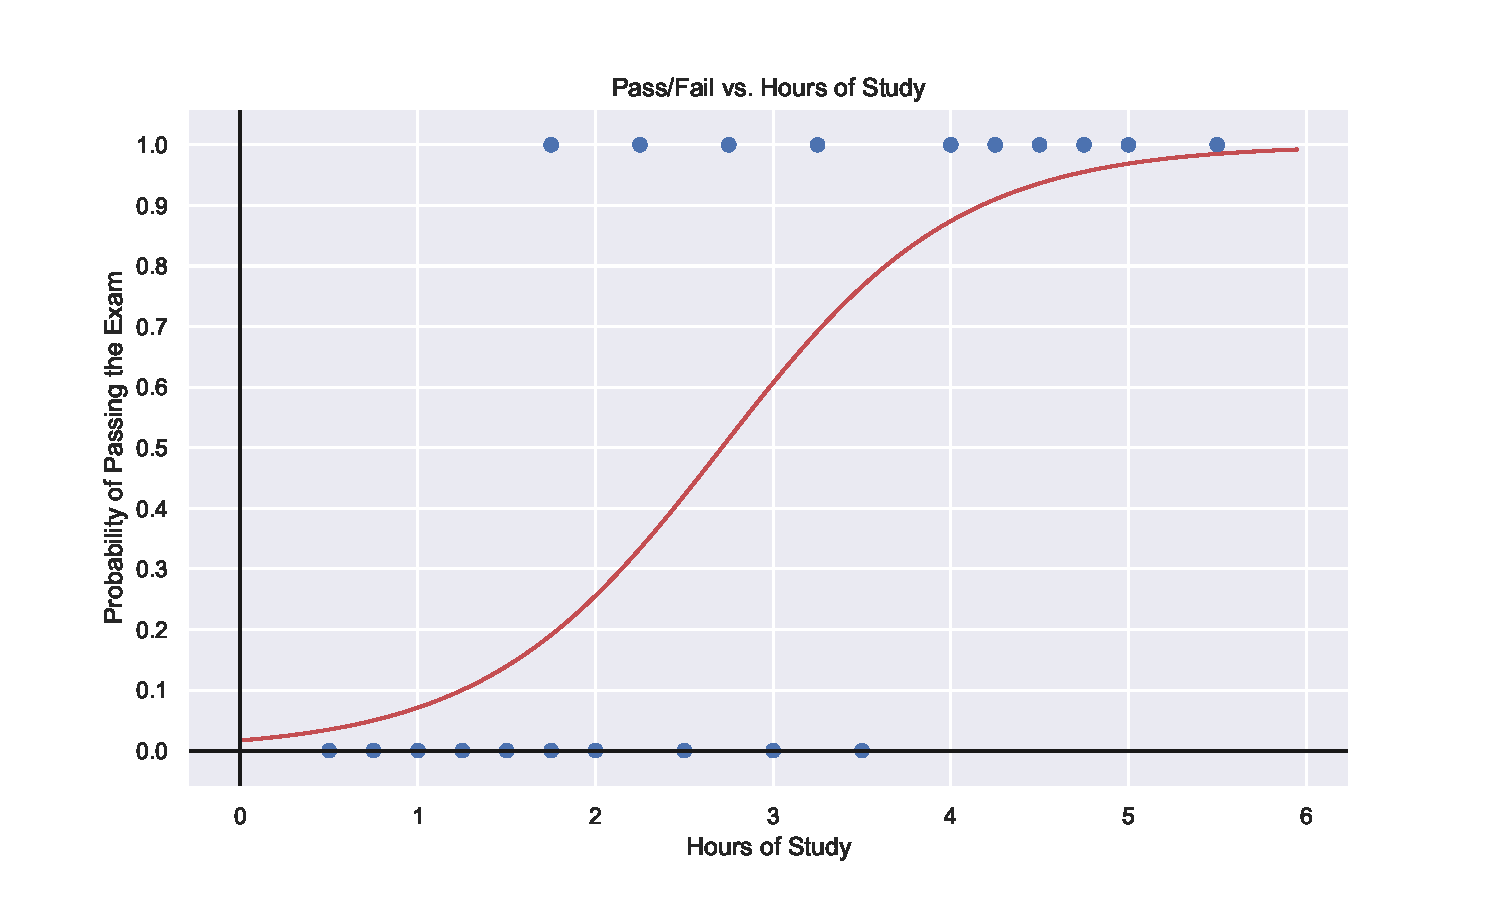
\epsfig{file=Figures/exam-probability.pdf, scale=0.7}
\caption{Probability of passing an exam versus hours of studying.}
\label{fig:exam-probability.pdf}
\end{figure}
\FloatBarrier

\subsection{Logistic Regression with SciKit-Learn}
In this section we discuss how linear regression is done in the SciKit-Learn environment.
We will improve on the previous example and study the data that is shown in Figure \ref{fig:exam-iq.csv} on
page \pageref{fig:exam-iq.csv}.
This \textsc{Csv} file contains data about a fictional exam.  The first column indicates whether the student
has passed or failed the exam.  A passed exam is encoded as the integer 1, while a failed exam is encoded as the integer 0.
The second column contains the number of hours that the student has studied for the exam.  The third column
contains the \href{https://en.wikipedia.org/wiki/Intelligence_quotient}{intelligence quotient}, abbreviated as
IQ.  To better understand the data, we first plot it.  This plot is shown in Figure \ref{fig:exam-iq.pdf} on
page \pageref{fig:exam-iq.pdf}.  The horizontal axis is used for the hours of study, while the vertical axis
shows the IQ of the student.  Students who have passed the exam are shown as blue dots, while those students
who have failed their exam are shown as red dots.

\begin{figure}[!ht]
\centering
\begin{Verbatim}[ frame         = lines, 
                  framesep      = 0.3cm, 
                  firstnumber   = 1,
                  labelposition = bottomline,
                  numbers       = left,
                  numbersep     = -0.2cm,
                  xleftmargin   = 0.8cm,
                  xrightmargin  = 0.8cm,
                ]
    Pass,Hours,IQ
    0,0.50,110
    0,0.75,95
    0,1.00,118
    0,1.25,97
    0,1.50,100
    0,1.75,110
    0,1.75,115
    1,2.00,104
    1,2.25,120
    0,2.50,98
    1,2.75,118
    0,3.00,88
    1,3.25,108
    0,3.50,125
    1,4.00,109
    1,4.25,110
    1,4.50,112
    1,4.75,97
    1,5.00,102
    1,5.50,109
\end{Verbatim}
\vspace*{-0.3cm}
\caption{Results of an exam given hours of study and IQ.}
\label{fig:exam-iq.csv}
\end{figure}

When we inspect the diagram shown in Figure \ref{fig:exam-iq.pdf} we see that there are two outliers: There is
one student who failed although he has an IQ of 125 and he did study for $3.5$ hours.  Maybe he was still drunk
when he had to write the exam.  There is also a student with an IQ of 104 who did pass while only studying for
$2$ hours.  He just might have gotten lucky. We expect logistic regression to classify all other students
correctly.

\begin{figure}[!th]
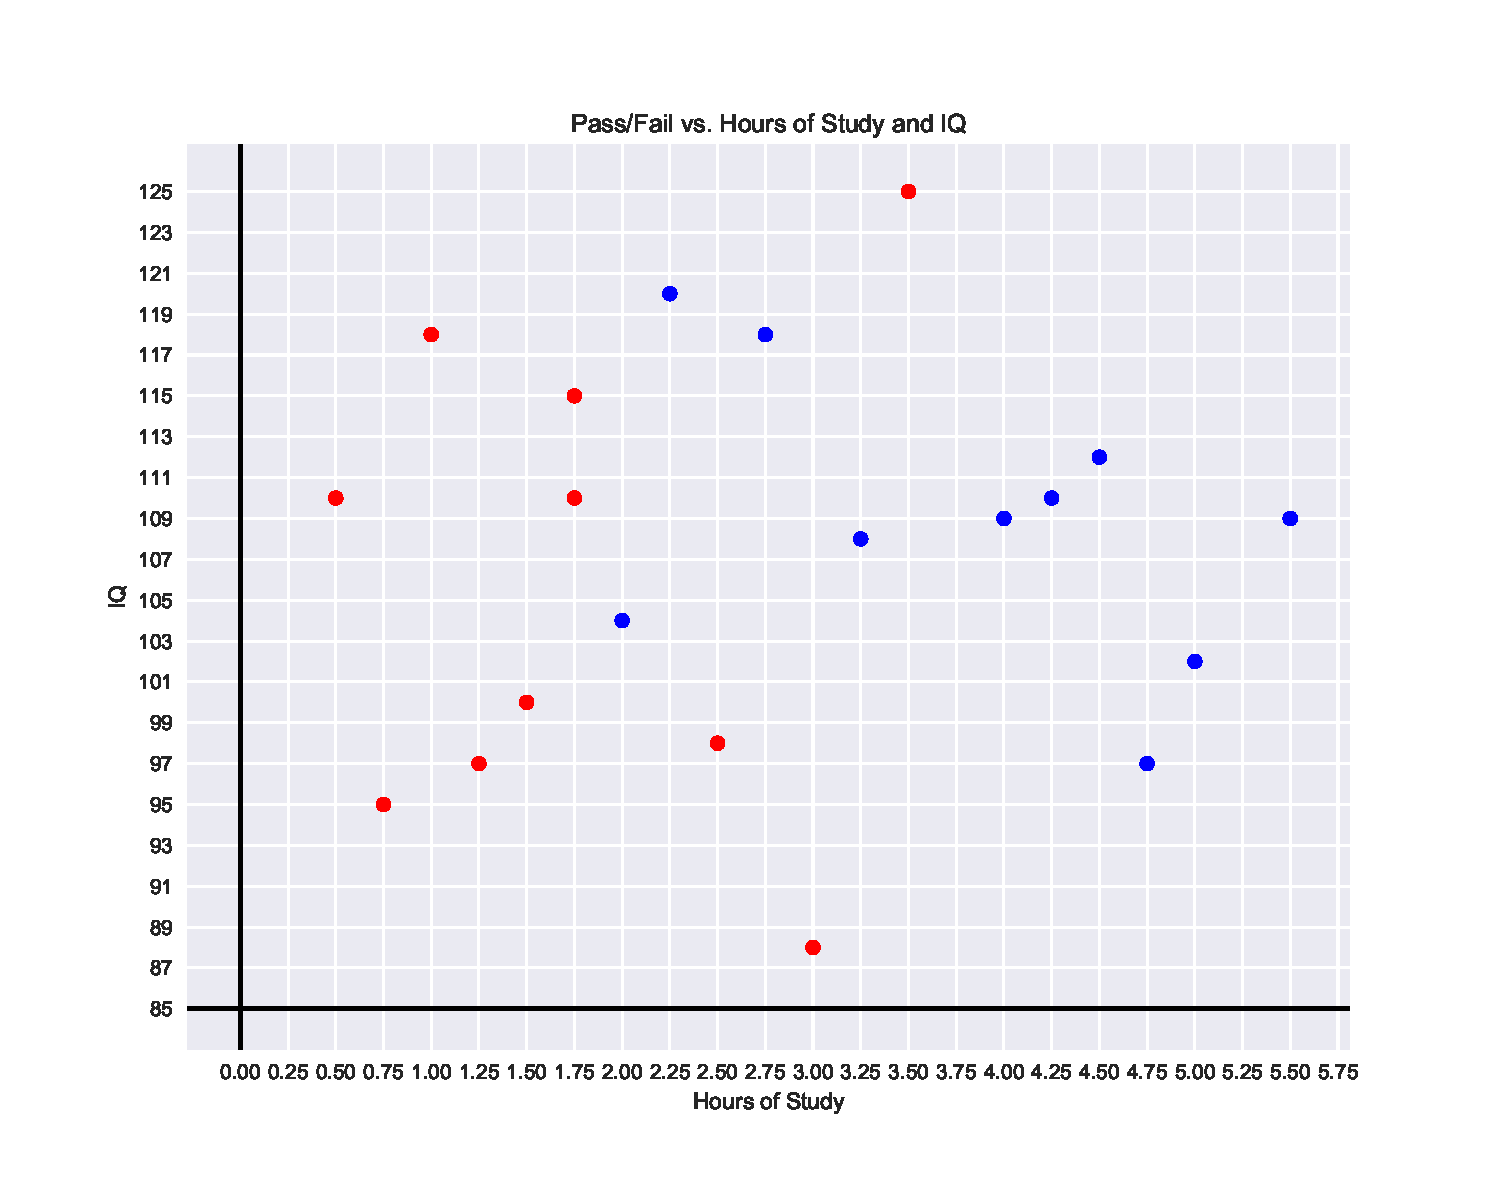
\epsfig{file=Figures/exam-iq.pdf, scale=0.6}
\caption{Probability of passing an exam versus hours of studying.}
\label{fig:exam-iq.pdf}
\end{figure}



\begin{figure}[!ht]
\centering
\begin{Verbatim}[ frame         = lines, 
                  framesep      = 0.3cm, 
                  firstnumber   = 1,
                  labelposition = bottomline,
                  numbers       = left,
                  numbersep     = -0.2cm,
                  xleftmargin   = 0.8cm,
                  xrightmargin  = 0.8cm,
                  commandchars  = \\\{\},
                  codes         = {\catcode`$=3\catcode`^=7\catcode`_=8}
                ]
    import numpy                as np
    import pandas               as pd
    import sklearn.linear\_model as lm
    
    ExamDF = pd.read\_csv('exam-iq.csv')
    X      = np.array(ExamDF[['Hours','IQ']])
    Y      = np.array(ExamDF['Pass'], dtype=float)
    model  = lm.LogisticRegression(C=10000, tol=1e-6, solver='newton-cg')
    M      = model.fit(X, Y)
    \(\vartheta_0\)     = M.intercept\_[0]
    \(\vartheta_1, \vartheta_2\) = M.coef\_[0]
    errors = np.sum(np.abs(Y - model.predict(X)))
    print((len(Y) - errors) / len(Y))
\end{Verbatim}
\vspace*{-0.3cm}
\caption{Logistic Regression using SciKit-Learn}
\label{fig:Logistic-Regression-with-SciKit-Learn.ipynb}
\end{figure}
\FloatBarrier

Figure \ref{fig:Logistic-Regression-with-SciKit-Learn.ipynb} on page
\pageref{fig:Logistic-Regression-with-SciKit-Learn.ipynb} shows a \textsl{Python} script that creates a
logistic regression classifier with the help of the SciKit-Learn package.
\begin{enumerate}
\item In the first three lines we import the necessary modules.
      The support for logistic regression is located in the module
      \texttt{sklearn.linear\_model}.
\item In line 5, the data from the file ``\texttt{exam-iq.csv}'' is read as a Pandas
      \href{https://pandas.pydata.org/pandas-docs/stable/reference/api/pandas.DataFrame.html}{DataFrame}.
\item Line 6 creates the feature matrix \texttt{X} by extracting the two independent variables ``\texttt{Hours}''
      and ``\texttt{IQ}''.
\item Line 7 extracts the dependent variable ``\texttt{Pass}''.  Since this variable is stored as an integer in
      the \textsc{Csv} file, we convert it into a floating point number.  This is necessary because the method
      \texttt{fit} that we use later expects the dependent variable to be encoded as a floating point number.
\item Line 8 creates an object of class \texttt{LogisticRegression}.  This object is initialized with a number
      of parameters:
      \begin{enumerate}
      \item \texttt{C} specifies the amount of \blue{regularization}.  We will discuss the concept of
            regularization later when we discuss \blue{polynomial logistic regression in the next section}.
            In this example we do not need any regularization.  Setting $C$ to a high value like $10\,000$
            prevents regularization.
      \item \texttt{tol} is the tolerance that specifies when the iterative algorithm to maximize the
            log-likelihood should stop.
      \item \texttt{solver} specifies the numerical method that is used to find the maximum of the
            log-likelihood. By choosing ``\texttt{newton-cg}'' we specify that the
            \href{https://en.wikipedia.org/wiki/Conjugate_gradient_method}{conjugate gradient}
            method should be used.  This method is more sophisticated than gradient descent, but as this is not
            a course on numerical optimization we do not have the time to discuss it.
      \end{enumerate}
\item All the real work is happening in line 9, because there we use the method \texttt{fit} to create the
      logistic regression model.
\item The next two lines are needed to extract the coefficients $\vartheta_0$, $\vartheta_1$, and $\vartheta_2$
      that specify the logistic model.      
      According to the model we have learned, the probability $P(h)$ that a student, who has learned for $h$
      hours and has an IQ of $q$, will pass the exam, is given as 
      $$ P(Y=1|h,q) = S(\vartheta_0 + \vartheta_1 \cdot h + \vartheta_2 \cdot q) $$
      In general, the model predicts that she will pass the exam if
      $$ \vartheta_0 + \vartheta_1 \cdot h + \vartheta_2 \cdot q \geq 0. $$
      This can be rewritten as follows:
      $$  q \geq -\frac{\vartheta_0 + \vartheta_1 \cdot h}{\vartheta_2}. $$
      The \blue{decision boundary} are those values of $(h, q)$ such that $P(h, q) = \frac{1}{2}$.  This set of
      values satisfies the linear equation
      $$  q = -\frac{\vartheta_0 + \vartheta_1 \cdot h}{\vartheta_2}. $$
      We have plotted this decision boundary as a green line in Figure \ref{fig:exam-iq-boundary.pdf} on page
      \pageref{fig:exam-iq-boundary.pdf}.  Everybody who is located to the right of this line is predicted to pass the exam,
      while everybody who is located to the left is predicted to fail.


\begin{figure}[!th]
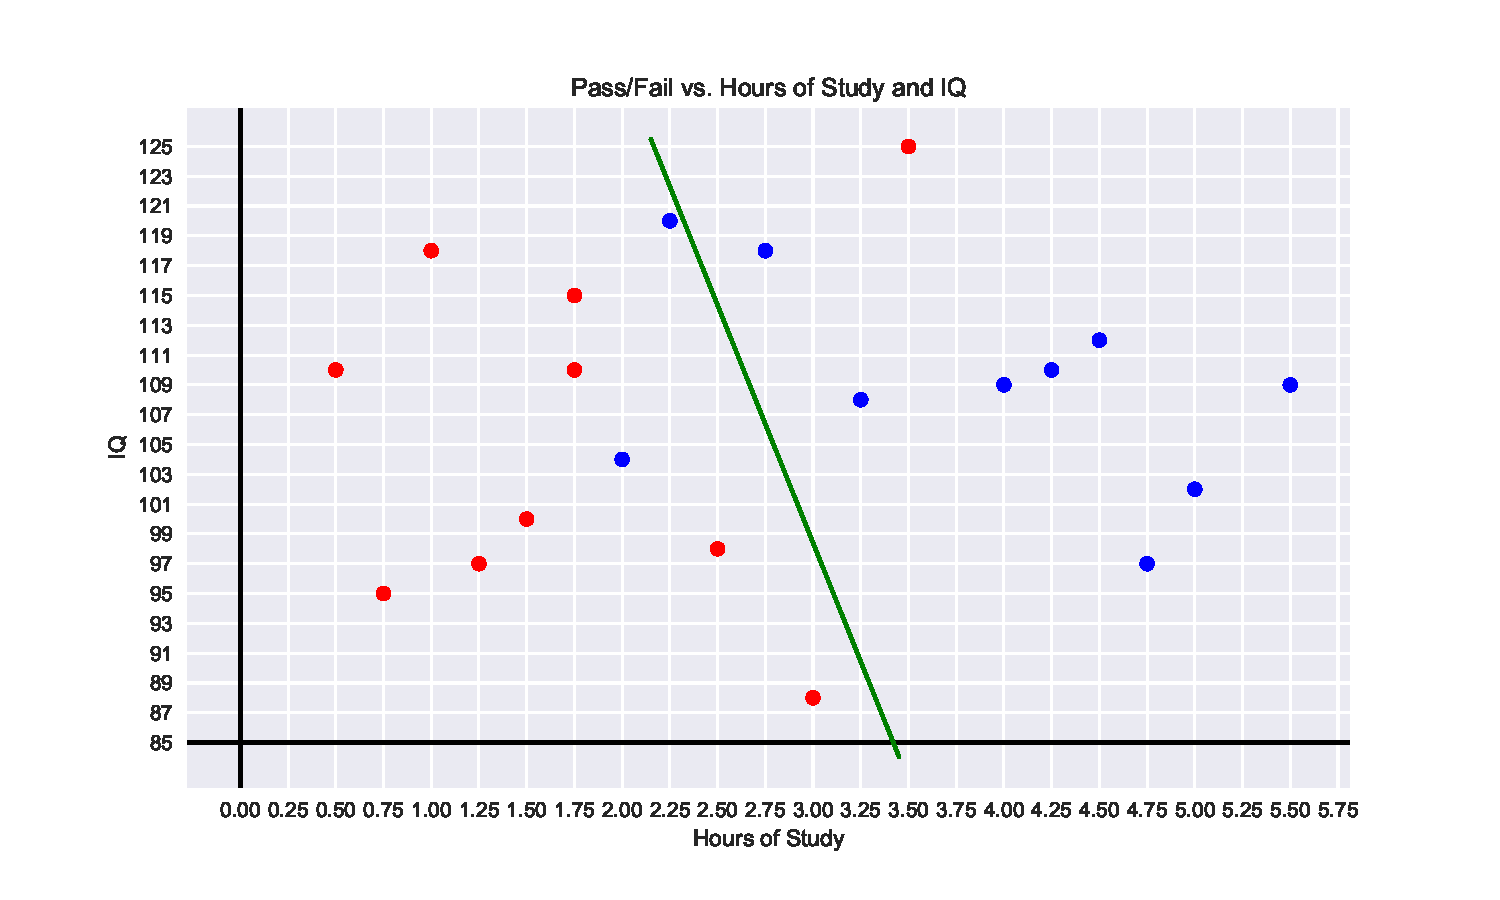
\epsfig{file=Figures/exam-iq-boundary.pdf, scale=0.6}
\caption{Probability of passing an exam versus hours of studying.}
\label{fig:exam-iq-boundary.pdf}
\end{figure}
\FloatBarrier
\item Line 12 computes the number of data for which the predictions of the model are wrong.
      The method $\texttt{predict}(X)$ takes a design matrix $X$.  Each row of $X$ is assumed to be a feature
      vector. It creates a prediction vector.  The $i$-th entry of this vector is $1$ if the model predicts a
      pass for the $i$-th student.  Otherwise this entry is $0$.
\item Line 13 prints the accuracy.  As Figure \ref{fig:exam-iq-boundary.pdf} shows, 3 examples have been
      miss-predicted.  Two of these examples where bound to be miss-predicted, but the fact that the student
      with an IQ of 120 who has studied for $2.25$ hours has also been miss-predicted is disappointing.
      The reason is that logistic regression does not maximize the accuracy but rather
      maximizes the log-likelihood.  Later, we will discuss so called 
      \blue{support vector machines}.  Often, a support vector machine is able to achieve a higher accuracy
      than logistic regression.  However, support vector machines are also more complicated than logistic regression.
 \end{enumerate}
The jupyter notebook containing the computation discussed previously can be found at my \href{https://github.com/karlstroetmann/Artificial-Intelligence}{github repository}:
\\[0.2cm]
\hspace*{1.3cm}
\href{https://github.com/karlstroetmann/Artificial-Intelligence/blob/master/Python/Logistic-Regression-with-SciKit-Learn.ipynb}
{Artificial-Intelligence/blob/master/Python/Logistic-Regression-with-SciKit-Learn.ipynb}

\exercise 
The file \href{https://github.com/karlstroetmann/Artificial-Intelligence/blob/master/Python/iris.csv}{iris.csv}
contains the sizes of both the \href{https://en.wikipedia.org/wiki/Sepal}{sepals} and the
\href{https://en.wikipedia.org/wiki/Pepal}{petals} of three different specimen of the iris flower.  The
data is described in more detail \href{https://en.wikipedia.org/wiki/Iris_flower_data_set}{here}. 
Use logistic regression to predict whether a given plant is of the species
\href{https://en.wikipedia.org/wiki/Iris_setosa}{iris setosa} (Deutsch: Borsten-Schwertlilie),
\href{https://en.wikipedia.org/wiki/Iris_virginica}{iris virginica}\footnote{
This plant is native to North America and hence has no German name.}, or
\href{https://en.wikipedia.org/wiki/Iris_versicolor}{iris versicolor} (Deutsch: Verschiedenfarbige Schwertlilie).
As logistic regression is only able to distinguish between two different classes, you
have to build three different classifiers:
\begin{itemize}
\item The first classifier is able to distinguish \blue{iris setosa} from other irises. 
\item The second classifier is able to distinguish \blue{iris virginica} from other irises. 
\item The third classifier is able to distinguish \blue{iris versicolor} from other irises. 
\end{itemize}
Your task is to implement these classifiers and to evaluate their accuracy.  
You should  divide the data randomly into a \blue{training dataset}, which is used for computing the
coefficients of logistic regression and a \blue{test dataset}, which you should only use to predict the
accuracy of your model.  To this end, the function
\\[0.2cm]
\hspace*{1.3cm}
\href{https://scikit-learn.org/stable/modules/generated/sklearn.model_selection.train_test_split.html}{\texttt{sklearn.model\_selection.train\_test\_split}}
\\[0.2cm]
might be useful.  Once you have created these classifiers, proceed to implement a classifier that inputs a
feature vector and that outputs the class of the iris flower as a string.  If you do this correctly, you can
achieve an accuracy that exceeds $95\%$.
\eox

\section{Polynomial Logistic Regression}
Sometimes logistic regression does not work because the data is not \blue{linearly separable}.  For example,
Figure \ref{fig:fake-data.pdf} on page \pageref{fig:fake-data.pdf} shows a classification problem where we have
two features $x$ and $y$ and, obviously, it is not possible to separate the blue dots from the red dots by a
vertical line.

\begin{figure}[!th]
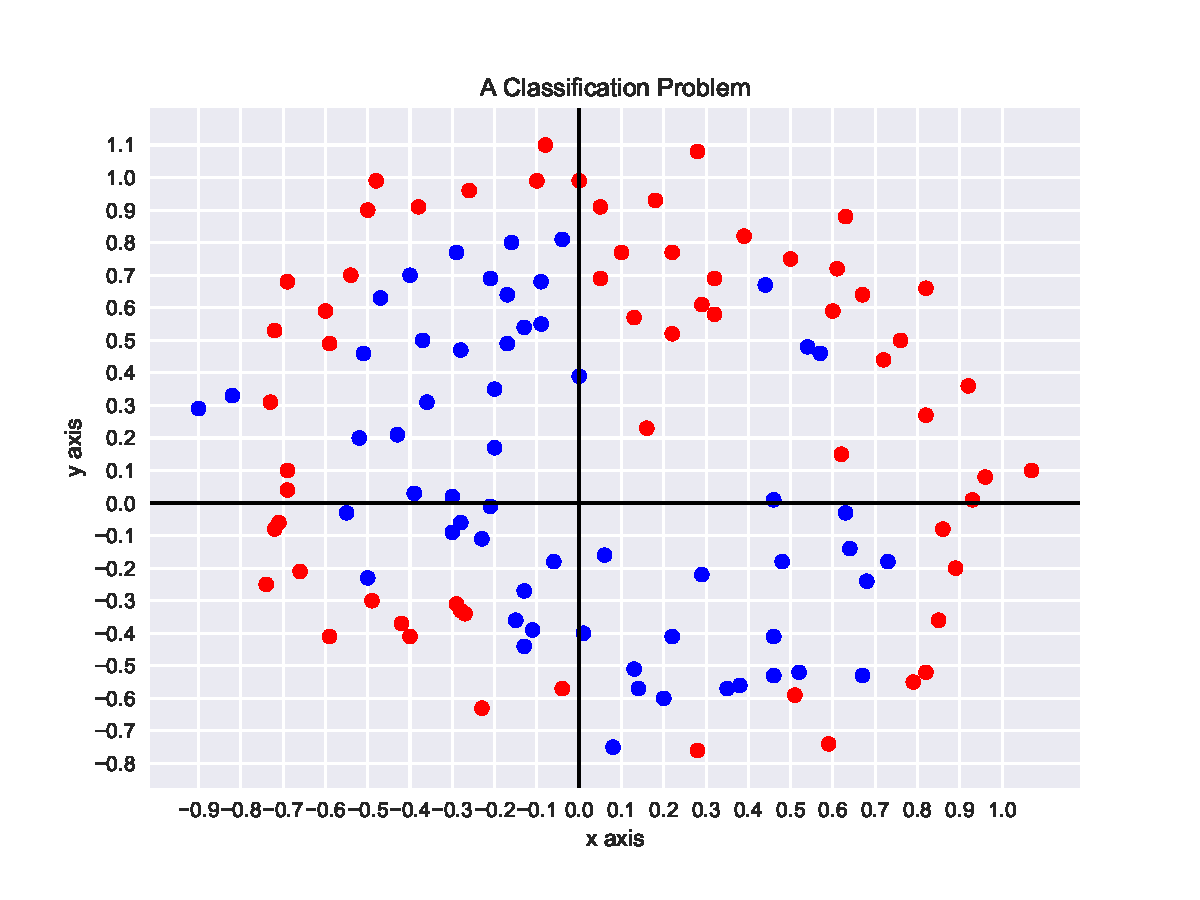
\epsfig{file=Figures/fake-data.pdf, scale=0.8}
\caption{Some fake data.}
\label{fig:fake-data.pdf}
\end{figure}

If we try to separate the data in Figure \ref{fig:fake-data.pdf} by logistic regression, we get the result
shown in Figure \ref{fig:fake-data-line.pdf} on page \pageref{fig:fake-data-line.pdf}.  The data points above
the green line are classified as red, while the data points below the green line are classified as blue.  The
accuracy achieved is about $61\%$, so more than $38\%$ of the data have been miss-classified.

\begin{figure}[!th]
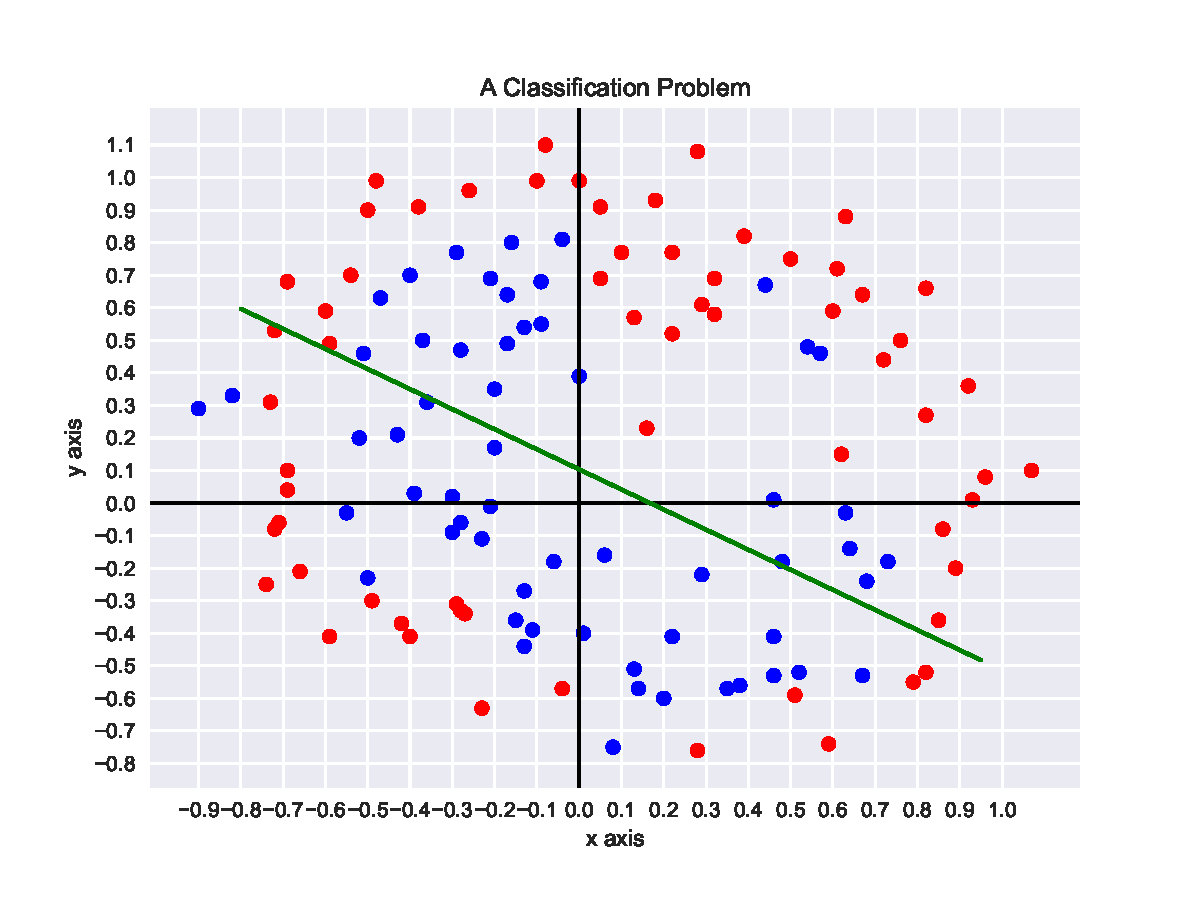
\epsfig{file=Figures/fake-data-line.pdf, scale=0.8}
\caption{Fake data with linear decision boundary.}
\label{fig:fake-data-line.pdf}
\end{figure}

We can arrive at a better model if we extend our data with \blue{second order polynomial features}, i.e. we will not only
consider the features $x$ and $y$ but also use $x^2$, $y^2$, and $x \cdot y$ as features.  Then the resulting
\blue{decision boundary} will be a \href{https://en.wikipedia.org/wiki/Conic_section}{conic section}, i.e.~it
might be an \href{https://en.wikipedia.org/wiki/Ellipse}{ellipse}, a
\href{https://en.wikipedia.org/wiki/Parabola}{parabola}, or a
\href{https://en.wikipedia.org/wiki/Hyperbola}{hyperbola}. 
Figure \ref{fig:Polynomial-Logistic-Regression.ipynb-quadratic} on page
\pageref{fig:Polynomial-Logistic-Regression.ipynb-quadratic} shows a \textsl{Python} script that reads the fake
data shown in Figure \ref{fig:fake-data.pdf}, adds second order polynomial features to this data and then
performs linear regression.


\begin{figure}[!ht]
\centering

\begin{minted}[ frame         = lines, 
                framesep      = 0.3cm, 
                firstnumber   = 1,
                numbers       = left,
                numbersep     = -0.2cm,
                xleftmargin   = 0.8cm,
                xrightmargin  = 0.8cm,
              ]{python3}
    import numpy  as np
    import pandas as pd
    import sklearn.linear_model as lm
    from sklearn.model_selection import train_test_split
    
    DF = pd.read_csv('fake-data.csv')
    X  = np.array(DF[['x','y']])
    Y  = np.array(DF['class'])
    
    X_train, X_test, Y_train, Y_test = train_test_split(X, Y, test_size=0.2, random_state=1)
    
    def logistic_regression(X_train, Y_train, X_test, Y_test, reg=10000):
        model    = lm.LogisticRegression(C=reg, tol=1e-6, solver='newton-cg')
        M        = model.fit(X_train, Y_train)
        score    = M.score(X_train, Y_train)
        yPredict = M.predict(X_test)
        accuracy = np.sum(yPredict == Y_test) / len(Y_test)
        return M, score, accuracy
    
    def extend(X):
        n  = len(X)
        fx = np.reshape(X[:,0], (n, 1))
        fy = np.reshape(X[:,1], (n, 1))
        return np.hstack([fx, fy, fx*fx, fy*fy, fx*fy])
    
    X_train_quadratic, X_test_quadratic = extend(X_train), extend(X_test)
    logistic_regression(X_train_quadratic, Y_train, X_test_quadratic, Y_test)
\end{minted}

\caption{A script for second order logistic regression.}
\label{fig:Polynomial-Logistic-Regression.ipynb-quadratic}
\end{figure}

\begin{enumerate}
\item The first three lines import the modules needed for this task.
\item As we want to split our data into a \blue{training set} and a \blue{test set}, we import the function
      \texttt{train\_test\_split} from \texttt{sklearn.model\_selection}.
\item Line 6 reads the data from the file ``\texttt{fake-data.csv}''.
\item Line 7 and 8 extract the independent variables ``\texttt{x}'' and ``\texttt{y}'' and the dependent
      variable ``\texttt{class}'' and stores them in the \blue{design matrix} \texttt{X} and the vector
      \texttt{Y}, respectively.
\item Line 10 splits the data into a \blue{training set} and a \blue{test set}.  We allocate $20\%$ of our data
      to the test set, while the remaining $80\%$ are used as training data.
      In order to be able to reproduce our results, we set \texttt{random\_state} to a fixed value.
      This forces the random number generator to always produce the same split of the data.
\item Line 12 defines the function \texttt{logistic\_regression}.  This function takes 5 arguments.
      \begin{enumerate}
      \item \texttt{X\_train} and \texttt{Y\_train} are the training data.
      \item \texttt{X\_test} and \texttt{Y\_} are the test data.
      \item \texttt{reg} is a \blue{regularization} parameter.  By default this parameter is set to a high
            value.  Setting this parameter to a high value ensures that there is no regularization.
            The default is to use next to no regularization.
      \end{enumerate}
      The function returns a triple of the form $(M, \mathtt{score}, \mathtt{accuracy})$ where
      \begin{enumerate}
      \item $M$ is the model that has been found.
      \item \texttt{score} is the fraction of data points from the training set that have been
            classified correctly.
      \item \texttt{accuracy} is the fraction of data points from the test set that have been
            classified correctly.
      \end{enumerate}
\item The function $\texttt{extend}(X)$ takes a design matrix $X$ as its argument.  In order to keep the
      implementation of this function simple, we assume that $X$ has just two features, i.e.~the matrix
      $\texttt{X}$ has shape $(n, 2)$ where $n$ is the number of rows of $X$.
      \begin{enumerate}
      \item We extract the two features of \texttt{X} in line 22 and 23.
      \item In line 24 the new feature matrix is created by stacking the original features \texttt{fx} and
            \texttt{fy} together with the new features $\mathtt{fx}^2$, $\mathtt{fy}^2$, $\mathtt{fx} \cdot \mathtt{fy}$, 
      \end{enumerate}
\item Line 26 extends both the training set and the test set with second order features.
\item Line 27 performs logistic regression using the new features.
      The use of second order feature improves the accuracy on the training set to $84\%$, while the accuracy
      on the test set improves to $76\%$.
      Figure \ref{fig:fake-data-ellipse.pdf} on page \pageref{fig:fake-data-ellipse.pdf} shows the resulting
      decision boundary.
\end{enumerate}


\begin{figure}[!th]
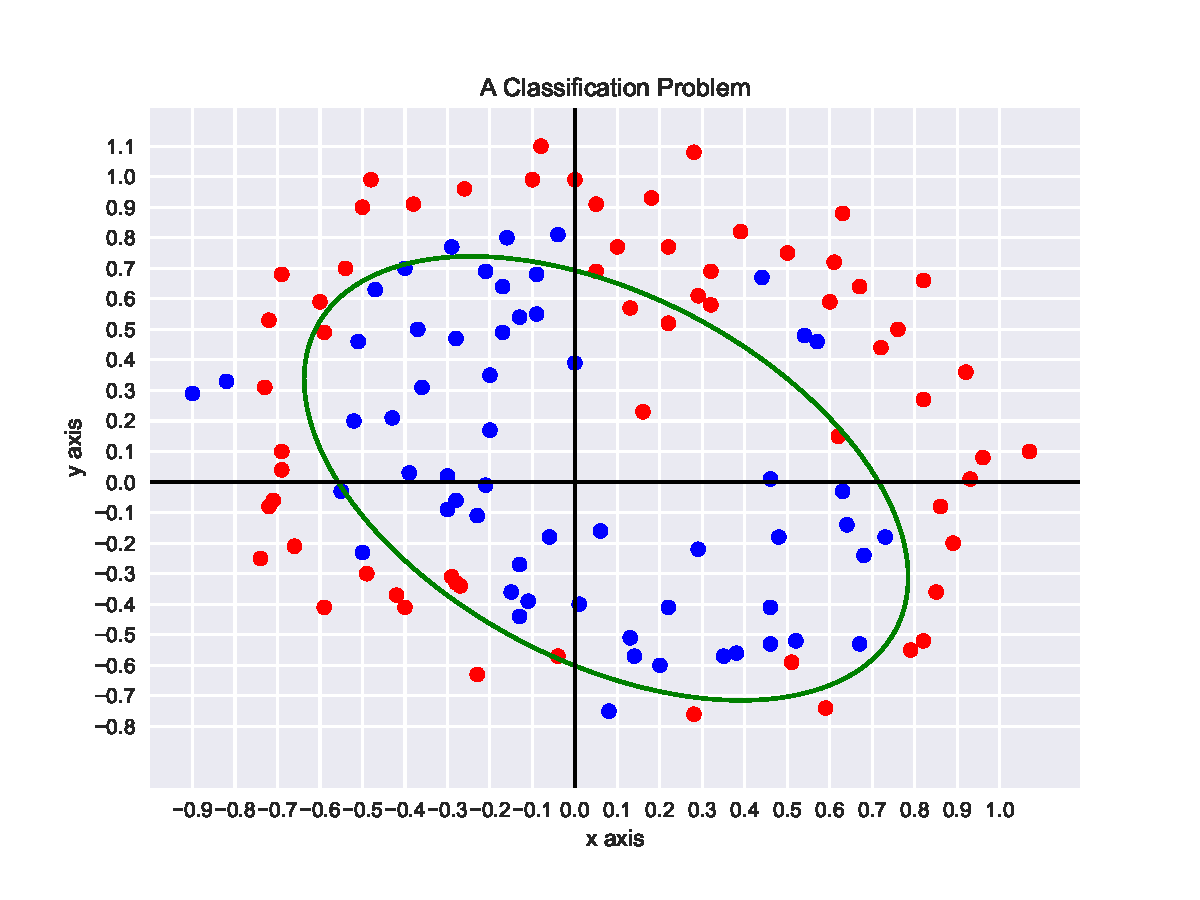
\epsfig{file=Figures/fake-data-ellipse.pdf, scale=0.8}
\caption{Elliptical decision boundary for fake data.}
\label{fig:fake-data-ellipse.pdf}
\end{figure}


As adding second order features has increased the accuracy considerably, we proceed to add higher order features.
Figure \ref{fig:Polynomial-Logistic-Regression.ipynb-quartic} on page
\pageref{fig:Polynomial-Logistic-Regression.ipynb-quartic} shows how we can add arbitrary polynomial features
of higher degree.  This script is a continuation of the script shown in Figure \ref{fig:Polynomial-Logistic-Regression.ipynb-quadratic}.

\begin{figure}[!th]
  \centering

\begin{minted}[ frame         = lines, 
                framesep      = 0.3cm, 
                firstnumber   = 1,
                numbers       = left,
                numbersep     = -0.2cm,
                xleftmargin   = 0.8cm,
                xrightmargin  = 0.8cm,
              ]{python3}
    from sklearn.preprocessing import PolynomialFeatures

    quartic = PolynomialFeatures(4, include_bias=False)
    X_train_quartic = quartic.fit_transform(X_train)
    X_test_quartic  = quartic.fit_transform(X_test)

    logistic_regression(X_train_quartic, Y_train, X_test_quartic, Y_test)
\end{minted}

\caption{Polynomial Logistic Regression.}
\label{fig:Polynomial-Logistic-Regression.ipynb-quartic}
\end{figure}

\begin{enumerate}
\item Line 28 imports the function \texttt{PolynomialFeatures} from \texttt{sklearn.preprocessing}.
      This function can be used to add all polynomial features up to a given order.
      We do not need a bias term here as it is automatically added by the function \texttt{LogisticRegression}.
\item Line 30 creates an object that can be used to extend a design matrix with polynomial features up to degree 4
\item Line 31 and 32 extend the training set and the test set with all polynomial features up to degree 4.
\item When we perform logistic regression with these new features, we achieve an accuracy of $88.4\%$ on the
      training set.  However, the accuracy on the test set does not improve.
      Figure \ref{fig:fake-data-quartic.pdf} on page \pageref{fig:fake-data-quartic.pdf} shows the data with
      the resulting decision boundary.
\end{enumerate}
 
\begin{figure}[!th]
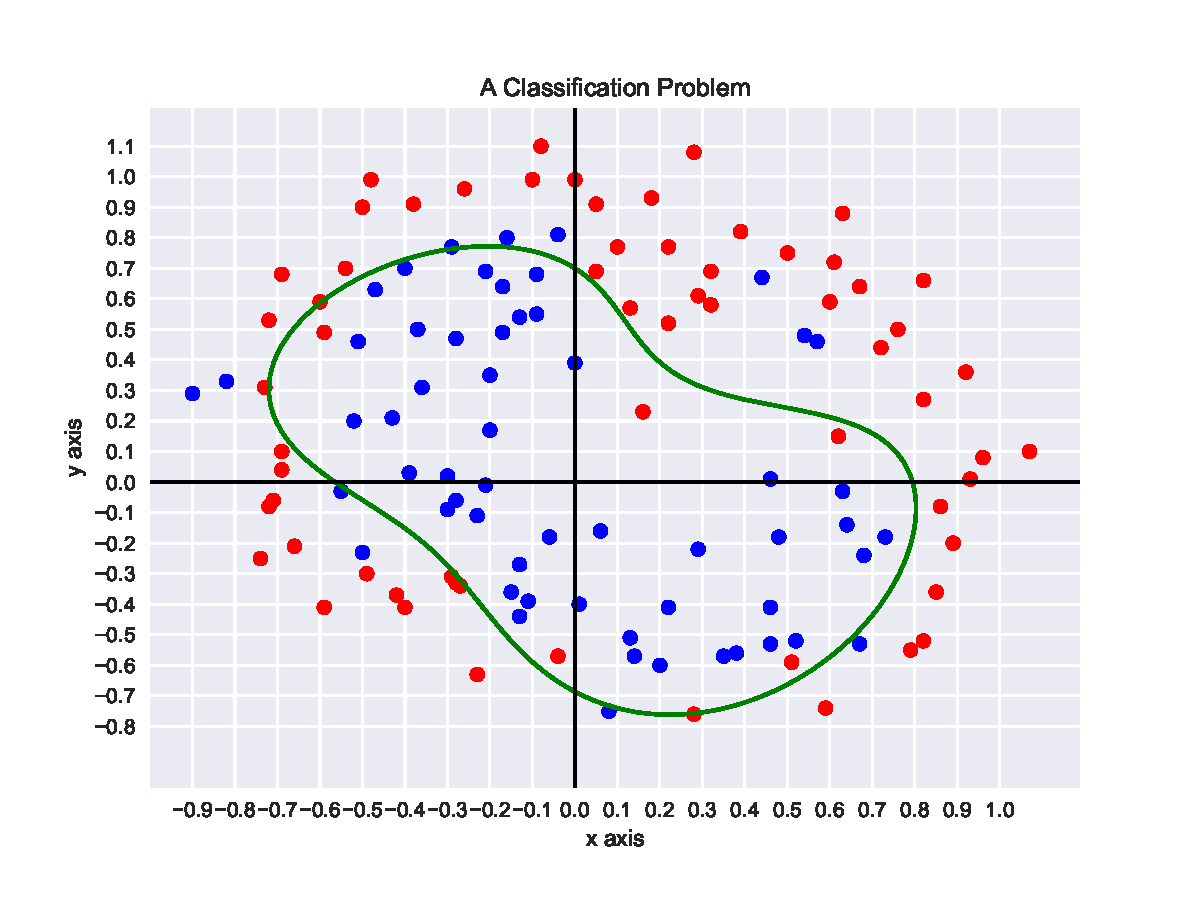
\epsfig{file=Figures/fake-data-quartic.pdf, scale=0.8}
\caption{Fake data with a decision boundary of fourth order.}
\label{fig:fake-data-quartic.pdf}
\end{figure}

Nothing stops us from cranking the order of the polynomial features to be added higher.
Figure \ref{fig:fake-data-14.pdf} on page \pageref{fig:fake-data-14.pdf} shows what happens when we include all
polynomial features up to a degree of 14.  In this case, we $100\%$ accuracy on the training set.  However, the
accuracy on the test set is only $80\%$.  Clearly, we are overfitting the data.

\begin{figure}[!th]
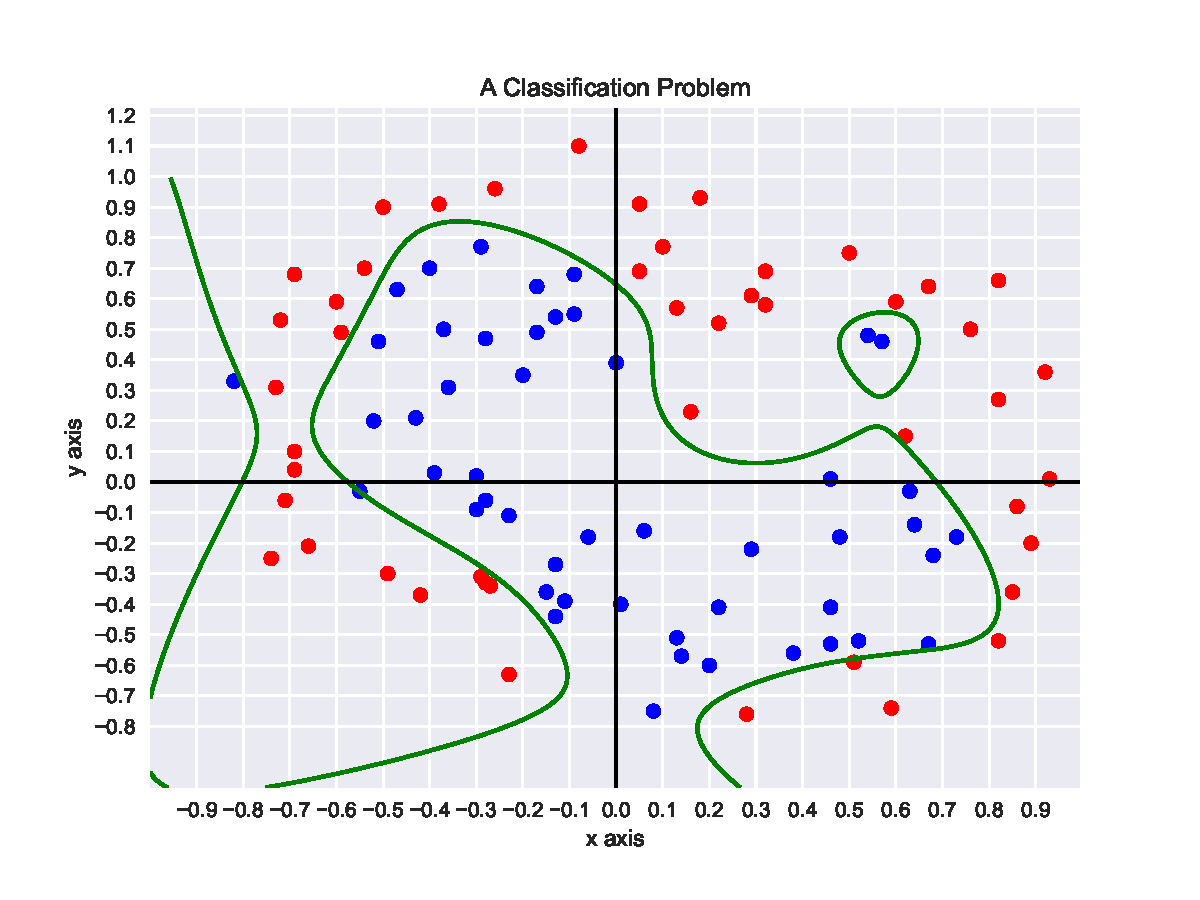
\epsfig{file=Figures/fake-data-14.pdf, scale=0.8}
\caption{Fake data with a decision boundary of order 14.}
\label{fig:fake-data-14.pdf}
\end{figure}

In order to combat overfitting we need to \blue{regularize}, i.e.~we need to penalize high values of the
parameters.  If we lower the regularization parameter down to $100$, then the accuracy on the training set
drops down to $89.6\%$, but the accuracy on the test set increases to $88\%$.  The resulting decision boundary
is shown in Figure \ref{fig:fake-data-14-reg.pdf} on page \pageref{fig:fake-data-14-reg.pdf}.  Clearly, this
decision boundary looks less complicated than the boundary shown in Figure \ref{fig:fake-data-14.pdf}.
Contrary to the previous figures, this figure shows all the data.  The previous figures had only shown the
training data.

\begin{figure}[!th]
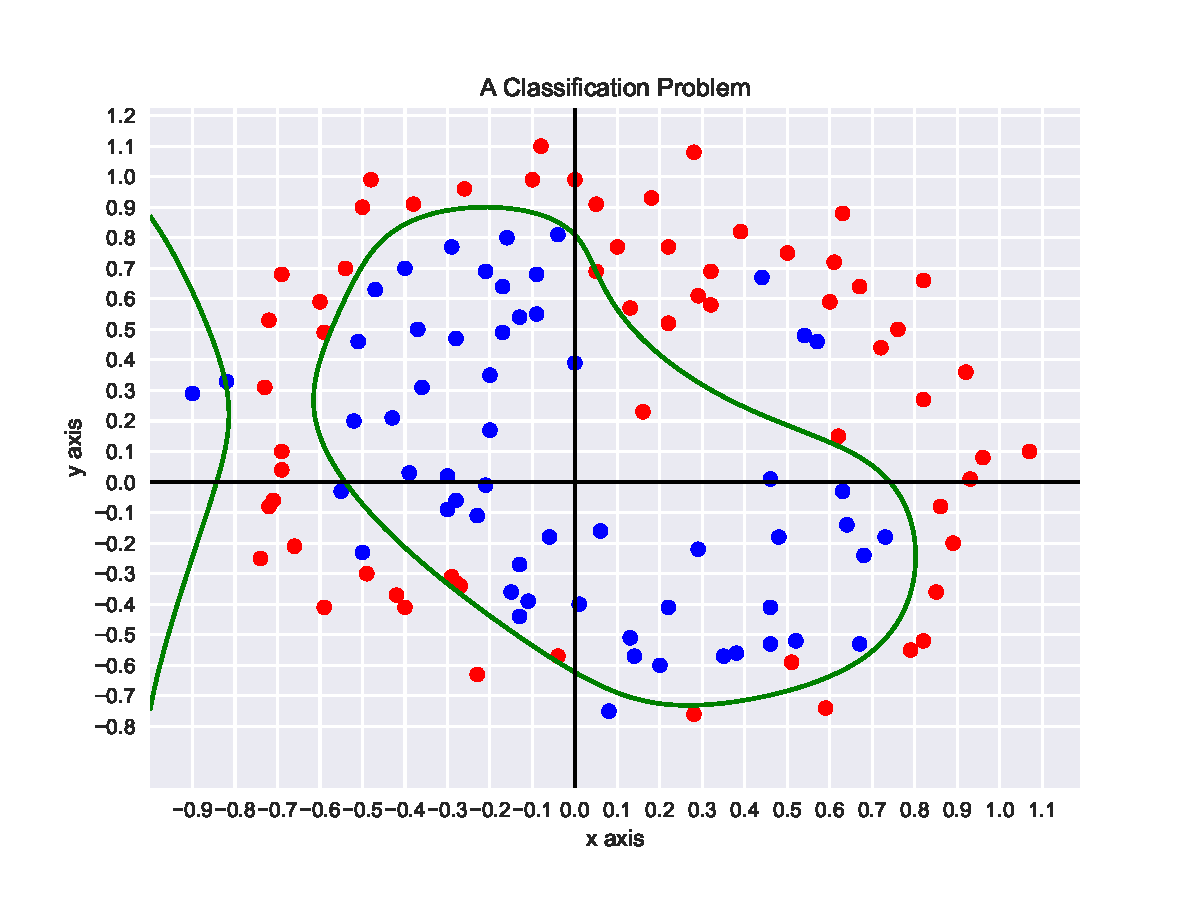
\epsfig{file=Figures/fake-data-14-reg.pdf, scale=0.8}
\caption{Fake data with a decision boundary of order 14, regularized.}
\label{fig:fake-data-14-reg.pdf}
\end{figure}

\exercise
\begin{enumerate}[(a)]
\item Assume that a design matrix $X$ has two features $x_1$ and $x_2$.  Given a natural number $n$, you want to
      extend this design matrix by adding all features of the form $x_1^{k_1} \cdot x_2^{k_2}$ such that
      $k_1 + k_2 \leq n$, i.e. you want to add all features up to a degree of $n$.
      How many features will the extended design matrix have?
\item Next, assume that the design matrix $X$ has three features $x_1$, $x_2$, and $x_3$.
      This time, you want to extend the design matrix by adding all features of the form
      $x_1^{k_1} \cdot x_2^{k_2} \cdot x_3^{k_3}$ where $k_1 + k_2 + k_3 \leq n$.
      How many features will the extended design matrix have in this case?
\item In the general case, the design matrix has $d$ features $x_1$, $\cdots$, $x_d$.  Assume you want to add all
     polynomial terms up to order $n$ as new features, i.e. you want to add all features of the form
     \\[0.2cm]
     \hspace*{1.3cm}
     $x_1^{k_1} \cdot x_2^{k_2} \cdot {\dots} \cdot x_d^{k_d}$ \quad such that $k_1 + k_2 + \cdots + k_d \leq n$.
     \\[0.2cm]
     How many features will the extended design matrix have in the general case?

     \textbf{Hint}:  You might find it helpful to revisit your old lecture notes on statistics.
     \eox
\end{enumerate}


\section{Naive Bayes Classifiers}
In this section we discuss \href{https://en.wikipedia.org/wiki/Naive_Bayes_classifier}{naive Bayes classifiers}.
Naive Bayes classifiers are an alternative method for classification which is appropriate in cases where the
features are not numerical but rather are categorical.  It starts with \href{https://en.wikipedia.org/wiki/Bayes%27_theorem}{Bayes' theorem}:
Assume we have some evidence $E$ about an object $o$ and want to know whether $o$ belongs to some class $C$.
Bayes' theorem tell us that the \blue{conditional probability} $P(C|E)$, i.e. the probability that $o$ has class $C$
given that we have observed the evidence $E$, is related to the conditional probability $P(E|C)$, which is the probability that we
observe the evidence $E$ given that $o$ has class $C$, in the following way:
\\[0.2cm]
\hspace*{1.3cm}
$\ds P(C|E) = \frac{P(E|C) \cdot P(C)}{P(E)}$.
\\[0.2cm]
This theorem is useful because often the conditional probability $P(E|C)$ that we observe some evidence $E$ in an object
$o$ of class $C$ is readily available, but the conditional probability $P(C|E)$ that an object has class $C$ if
we have observed the evidence $E$ is unknown.  In the context of machine learning the evidence $E$ is often
given as a list of features $f_1$, $\cdots$, $f_m$ that we are able to observe or compute.  In this case we
have to rewrite Bayes' theorem as follows:
\\[0.2cm]
\hspace*{1.3cm}
$\ds P(C\;|\;f_1 \wedge \cdots \wedge f_m) = \frac{P(f_1 \wedge \cdots \wedge f_m\;|\;C) \cdot P(C)}{P(f_1 \wedge \cdots \wedge f_m)}$.
\\[0.2cm]
In order to apply this form of Bayes' theorem to the problem of classification, we have to rewrite the expression
\\[0.2cm]
\hspace*{1.3cm}
$P(f_1 \wedge \cdots \wedge f_m\;|\;C)$.
\\[0.2cm]
In order to be able to do this, we need some theory which will be developed next.  The conditional probability
$P(A|B)$ that an event $A$ happens when it is already known that $B$ has happened is defined as 
\\[0.2cm]
\hspace*{1.3cm}
$\ds P(A|B) = \frac{P(A \wedge B)}{P(B)}$.
\\[0.2cm]
This equation can be rewritten as
\\[0.2cm]
\hspace*{1.3cm}
$P(A \wedge B) = P(A|B) \cdot P(B)$.
\\[0.2cm]
Because conditional probabilities are probabilities and hence obey all the laws for probabilities, this
equation is also true for conditional probabilities: 
\\[0.2cm]
\hspace*{1.3cm}
$P(A \wedge B\;|\;C) = P(A\;|\;B \wedge C) \cdot P(B\;|\;C)$.
\\[0.2cm]
This equation can be generalized to the so called \href{https://en.wikipedia.org/wiki/Chain_rule_(probability)}{chain rule of probability}:
\\[0.2cm]
\hspace*{1.2cm}
$
\begin{array}[t]{lcl}
       P(A_1 \wedge \cdots \wedge A_m \;|\;C) 
 & = & P(A_1 \wedge  \cdots \wedge A_{m-1}\;|\;A_{m} \wedge C) \cdot P(A_{m}\;|\;C) \\[0.2cm]
 & = & P(A_1 \wedge  \cdots \wedge A_{m-2}\;|\;A_{m-1} \wedge A_{m} \wedge C) \cdot P(A_{m-1} \;|\;A_m \wedge C)\cdot P(A_{m}\;|\;C) \\
 & = & \cdots \\
 & = &  P(A_1 \;|\; A_2 \wedge  \cdots \wedge A_{m} \wedge C) \cdot \,\dots\, \cdot P(A_{m-1} \;|\;A_m \wedge C)\cdot P(A_{m}\;|\;C) \\[0.2cm]
 & = & \prod\limits_{i=1}^m P(A_i \;|\; A_{i+1} \wedge  \cdots \wedge A_{m} \wedge C) 
\end{array}
$
\\[0.2cm]
Two events $A$ and $B$ are defined to be \href{https://en.wikipedia.org/wiki/Conditional_independence}{conditional independent}
given an event $C$ if and only if we have
\\[0.2cm]
\hspace*{1.3cm}
$P(A \;|\; C) = P(A \;|\; B \wedge C)$.
\\[0.2cm]
To put this equation differently, once we know that $C$ holds, when it comes to the estimating the probability of $A$,
then it does not matter whether $B$ holds or not.  Now the important assumption that a \blue{naive Bayes classifier} 
makes is that in order to estimate the class $C$ of an object $o$ that has features $f_1$, $\cdots$, $f_m$ it
is assumed that the features $f_1, \cdots, f_m$ are conditionally independent once the class is known.  In
most applications of naive Bayes classifiers this assumption is not true because there might be some weak
correlation between the features.  That explains why naive Bayes classifiers are called \blue{naive}.  Still,
in practise the conditional independence of the features given 
the class is often approximately true and therefore these classifiers are useful.  If we make the
assumption of conditional independence, then the probability $P(C\;|\; f_1 \wedge \cdots \wedge f_m)$ of an
object $o$ with features $f_1$, $\cdots$, $f_m$ to be of class $C$ is given as
\\[0.2cm]
\hspace*{1.3cm}
$
\begin{array}[t]{lcll}
      P(C\;|\; f_1 \wedge \cdots \wedge f_m) 
& = & \ds \frac{P(f_1 \wedge \cdots \wedge f_m \;|\; C) \cdot P(C)}{P(f_1 \wedge \cdots \wedge f_m)} \cdot P(C) \\[0.2cm]
& = & \ds \frac{\prod\limits_{i=1}^m P(f_i \;|\; f_{i+1} \wedge \cdots \wedge f_m \wedge C)}{P(f_1 \wedge \cdots \wedge f_m)} \cdot P(C) \\[0.4cm]
& = & \ds \frac{\prod\limits_{i=1}^m P(f_i \;|\; C)}{P(f_1 \wedge \cdots \wedge f_m)} \cdot P(C) 
\end{array}
$
\\[0.2cm]
In the last line of the previous chain of equations we have used the fact that the features $f_1$, $\cdots$,
$f_m$ are conditionally independent given $C$.  Now a naive Bayes classifier works as follows: 
Assume we have a set of $n$ classes $\mathcal{C} = \{ C_1, \cdots, C_n \}$ from which we have to choose the
class of an object $o$ given the features  $f_1$, $\cdots$, $f_m$.  We assume that $o$ has class $C_k$ if
and only if the probability $P(C_k\;|\; f_1 \wedge \cdots \wedge f_m)$ is maximal with respect to all classes
of $\mathcal{C}$.  In order to be able to specify this in a more formal
way, we define the \blue{$\arg\max$} function: Given a set $S$ and a function $f:S \rightarrow \mathbb{R}$ that has
exactly one maximum, we define
\\[0.2cm]
\hspace*{1.3cm}
$\arg\max\limits_{x \in S} f(x) := \texttt{arb}\Bigl(\bigl\{ x \in S \mid \forall y \in S: f(y) \leq f(x)\bigr\}\Bigr)$,
\\[0.2cm]
where the function $\texttt{arb}(M)$ returns an arbitrary element from the set $M$. 
Since we assume that $f$ has exactly one element on the set $S$, the expression 
$\arg\max\limits_{x \in S} f(x)$ is well defined.  To
put the definition of  $\arg\max\limits_{x \in S} f(x)$ differently, the idea is that
$\arg\max\limits_{x \in S} f(x)$ computes the value of $x$ that maximizes $f$.  Given the features  $f_1$, $\cdots$,
$f_m$, the naive Bayes classifier computes the most probable class as follows:
\\[0.2cm]
\hspace*{1.3cm}
$\ds \texttt{NaiveBayes}(f_1,\cdots,f_m) :=
  \arg\max\limits_{C \in \mathcal{C}}  \frac{\prod\limits_{i=1}^m P(f_i \;|\; C)}{P(f_1 \wedge \cdots \wedge f_m)} \cdot P(C) 
$
\\[0.2cm]
It is important to observe that the denominator $P(f_1 \wedge \cdots \wedge f_m)$ does not depend on the class
$C$.  As we only need to determine the class with the maximal probability, not the exact probability of the
class, we can simplify the definition by dropping this denominator.  Therefore the definition of the naive
Bayes classifier can be rewritten as follows:
\\[0.2cm]
\hspace*{1.3cm}
$\ds \texttt{NaiveBayes}(f_1,\cdots,f_m) :=
  \arg\max\limits_{C \in \mathcal{C}}  \left(\prod\limits_{i=1}^m P(f_i \;|\; C)\right) \cdot P(C) 
$
\\[0.2cm]
This equation can be implemented once we have a training set $T$ of objects with known classes:  
The probability $P(C)$ is the probability that an object $o$ has class $C$
if nothing else is known about this object.  $P(C)$ is estimated as the proportion of objects in $T$ that are
of class $C$:
\\[0.2cm]
\hspace*{1.3cm}
$ \ds P(C) \approx \frac{\texttt{card}\bigl(\{t \in T \;|\; \texttt{class}(t) = C \}\bigr)}{\texttt{card}(T)}$.
\\[0.2cm]
This expression is called the \blue{prior probability} of $C$ or sometimes just the \blue{prior} of $C$.
In this equation, given an object $t\in T$ the function $\texttt{class}(t)$ determines the class of the object
$t$, while $\texttt{card}(M)$ returns the number of elements of the set $M$.

Next, given a feature $f$ and a class $C$, we have to determine the \blue{conditional probability} that an
object of class $C$ exhibits the feature $f_i$, i.e. we have to determine $P(f_i \;|\; C)$.
This probability can be estimated as the proportion of those objects of class $C$ in the training set $T$ that
possess the feature $f$:
\\[0.2cm]
\hspace*{1.3cm}
$\ds P(f\;|\;C) \approx 
 \frac{\texttt{card}\bigl(\{t \in T \;|\; \texttt{class}(t) = C \wedge \texttt{has}(t, f) \}\bigr)}{
       \texttt{card}\bigl(\{t \in T \;|\; \texttt{class}(t) = C \}\bigr)} 
$
\\[0.2cm]
Here, for an object $t$ and a feature $f$ the expression $\texttt{has}(t, f)$ is true if and only if $t$ has
the feature $f$.

\subsection{Example: Spam Detection}
\href{https://en.wikipedia.org/wiki/Naive_Bayes_spam_filtering}{Spam detection} is an important application of
classification.  We will see in this subsection that naive Bayes classifiers work well for spam detection.
The directory
\\[0.2cm]
\hspace*{1.3cm}
\href{https://github.com/karlstroetmann/Artificial-Intelligence/tree/master/Python/EmailData}{
https://github.com/karlstroetmann/Artificial-Intelligence/tree/master/Python/EmailData}
\\[0.2cm]
contains 960 emails that are partitioned into four subdirectories:
\begin{enumerate}
\item \texttt{spam-train} contains 350 spam emails for training,
\item \texttt{ham-train}  contains 350 non-spam emails for training,
\item \texttt{spam-test}  contains 130 spam emails for testing,
\item \texttt{ham-test}   contains 130 non-spam emails for testing.
\end{enumerate}
This data has been collected by Ion Androutsopoulos.  Figure \ref{fig:Spam-Detection.ipynb-1} on page
\pageref{fig:Spam-Detection.ipynb-1} and \ref{fig:Spam-Detection.ipynb-2} on page
\pageref{fig:Spam-Detection.ipynb-2} show parts of the notebook 
\\[0.2cm]
\hspace*{1.3cm}
\href{https://github.com/karlstroetmann/Artificial-Intelligence/blob/master/Python/Spam-Detection.ipynb}{
https://github.com/karlstroetmann/Artificial-Intelligence/blob/master/Python/Spam-Detection.ipynb}.
\\[0.2cm]
This notebook implements a naive Bayes classifier for spam detection.  We proceed to discuss the details of its
implementation.



\begin{figure}[!ht]
\centering

\begin{minted}[ frame         = lines, 
                framesep      = 0.3cm, 
                firstnumber   = 1,
                numbers       = left,
                numbersep     = -0.2cm,
                xleftmargin   = 0.8cm,
                xrightmargin  = 0.8cm,
              ]{python3}
    import os
    import re
    import numpy as np
    import math

    from collections import Counter

    spam_dir_train = 'EmailData/spam-train/'
    ham__dir_train = 'EmailData/ham-train/'
    spam_dir_test  = 'EmailData/spam-test/'
    ham__dir_test  = 'EmailData/ham-test/'
    Directories    = [spam_dir_train, ham__dir_train, spam_dir_test, ham__dir_test]
    
    no_spam    = len(os.listdir(spam_dir_train))
    no_ham     = len(os.listdir(ham__dir_train))
    spam_prior = no_spam / (no_spam + no_ham)
    ham__prior = no_ham  / (no_spam + no_ham)

    def get_words(fn):
        file = open(fn)
        text = file.read()
        text = text.lower()
        return set(re.findall(r"[\w']+", text))

    def read_all_files(Directories):
        Words = Counter()
        for directory in Directories:
            for file_name in os.listdir(directory):
                Words.update(get_words(directory + file_name))
        return Words
    
    Word_Counter = read_all_files(Directories)
    Common_Words = { w for w, _ in Word_Counter.most_common(2500) }

    def get_common_words(fn):
        return get_words(fn) & Common_Words

    def count_commmon_words(directory):
        Words = Counter()
        for file_name in os.listdir(directory):
            Words.update(get_common_words(directory + file_name))
        return Words

    spam_counter = count_commmon_words(spam_dir_train)
    ham__counter = count_commmon_words(ham__dir_train)
\end{minted}

\caption{A Naive Bayes Classifier for Spam Detection: Part \texttt{I}}
\label{fig:Spam-Detection.ipynb-1}
\end{figure}

\begin{enumerate}
\item Initially we load a number of modules.  In addition to \texttt{numpy} and \texttt{math} these are
      \begin{enumerate}
      \item \texttt{os} to list the files in a directory.
      \item \texttt{re} for regular expressions.
      \end{enumerate}
\item We import the module
      \href{https://docs.python.org/2/library/collections.html#counter-objects}{\texttt{Counter}} from the package
      \texttt{collections}.  
      A \texttt{Counter} is a special type of dictionary that is well suited for counting objects.
\item We set some variables that would need to be adapted if this notebook would be used with a different set of
      Emails.
\item Using the function \texttt{listdir} from the module \texttt{os} we count the number of spam emails and
      the number of ham emails in the corresponding directories.  These numbers are than used to compute the
      prior probabilities for spam and ham.  In our example, the number of spam emails and the number of ham
      emails are both 350.  Therefore, the prior probability of an email to be spam is $\frac{1}{2}$ and the
      prior probability for ham is also $\frac{1}{2}$.
\item The function $\texttt{get\_words}(\texttt{fn})$ takes a filename $\texttt{fn}$ as its argument.  
      \begin{enumerate}
      \item It reads the specified file as a string of text.  
      \item This string of text is then converted to lower case.

            In our case the conversion to lower case would not be necessary as the emails that we use
            have been preprocessed and are already converted to lower case.
      \item The text string is split into a list of words using the function \texttt{findall}
            from the module \texttt{re}.  The regular expression
            \\[0.2cm]
            \hspace*{1.3cm}
            \texttt{r"[\symbol{92}w']+"}
            \\[0.2cm]
            specifies all strings that are made up of Unicode word characters and single quote characters.
            The list of words returned by \texttt{findall} is then converted to a set and returned.
      \end{enumerate}
\item The function \texttt{read\_all\_files} reads all files contained in the directories that are stored in
      the list \texttt{Directories}.  It returns a \texttt{Counter}.  For every word $w$ this counter contains the number of
      those files that contain $w$.  
      
      Given a counter $C$ and a set $S$, the function $C.\texttt{update}(S)$ increments the count of every
      element $x$ in $C$ that occurs in the set $S$.  For example, if
      \\[0.2cm]
      \hspace*{1.3cm}
      $C = \mathtt{Counter}(\{\mathtt{a}\colon 1, \mathtt{b}\colon 2, \mathtt{c}\colon 3\})$, 
      \\[0.2cm]
      then the call $C.\mathtt{update}(\{\mathtt{a}, \mathtt{d}\})$ changes the counter $C$ such that afterwards
      \\[0.2cm]
      \hspace*{1.3cm}
      $C = \mathtt{Counter}(\{\mathtt{a}\colon 2, \mathtt{b}\colon 2, \mathtt{c}\colon 3, \mathtt{d}\colon 1\})$.
\item \texttt{Word\_Counter} is a \texttt{Counter} object that contains the counts of all words that occur in
      any email.
\item \texttt{Common\_Words} is list of the 2500 most common words occurring in all emails.
\item The function $\texttt{get\_common\_words}(\texttt{fn})$ takes a filename $\texttt{fn}$ 
      as its argument.  It reads the specified file and returns set of all words in \texttt{Common\_Words} that
      are found in the specified file.  
\item The function \texttt{count\_common\_words} takes a \texttt{directory} as its argument.  It returns a 
      \texttt{Counter} that counts how often the words in \texttt{Common\_Words} occur in any of the files in
      \texttt{directory}.
\item We use this function to count how often the most common words occur in spam and ham emails.
      These counts are stored in the dictionaries \texttt{Spam\_Counter} and \texttt{Ham\_\_Counter}.
\end{enumerate}
The second part of our spam classifier is shown in Figure \ref{fig:Spam-Detection.ipynb-2} on page
\pageref{fig:Spam-Detection.ipynb-2} and is discussed below.


\begin{figure}[!ht]
\centering

\begin{minted}[ frame         = lines, 
                framesep      = 0.3cm, 
                firstnumber   = last,
                numbers       = left,
                numbersep     = -0.2cm,
                xleftmargin   = 0.8cm,
                xrightmargin  = 0.8cm,
              ]{python3}
    Spam_Probability = {}
    Ham__Probability = {}
    for w in Common_Words:
        Spam_Probability[w] = (Spam_Counter[w] + 1) / (no_spam + 1) 
        Ham__Probability[w] = (Ham__Counter[w] + 1) / (no_ham  + 1) 

    def spam_probability(fn):
        log_p_spam = 0.0
        log_p_ham  = 0.0
        words = get_common_words(fn)
        for w in Common_Words:
            if w in words:
                log_p_spam += math.log(Spam_Probability[w])
                log_p_ham  += math.log(Ham__Probability[w])
            else:
                log_p_spam += math.log(1.0 - Spam_Probability[w])
                log_p_ham  += math.log(1.0 - Ham__Probability[w])
        alpha = abs(min(log_p_spam, log_p_ham))
        if alpha > 400: # avoid overflow
            if log_p_spam < log_p_ham:
                return 0
            else:
                return 1
        p_spam = math.exp(log_p_spam + alpha) * spam_prior
        p_ham  = math.exp(log_p_ham  + alpha) * ham__prior
        return p_spam / (p_spam + p_ham)

    def precission_recall(spam_dir, ham_dir):
        TN = 0 # true negatives
        FP = 0 # false positives
        for email in os.listdir(spam_dir):
            if spam_probability(spam_dir + email) > 0.5:
                TN += 1
            else:
                FP += 1
        FN = 0 # false negatives
        TP = 0 # true positives
        for email in os.listdir(ham_dir):
            if spam_probability(ham_dir + email) > 0.5:
                FN += 1
            else:
                TP += 1
        precision = TP / (TP + FP)
        recall    = TP / (TP + FN)
        accuracy  = (TN + TP) / (TN + TP + FN + FP)
        return precision, recall, accuracy
\end{minted}
    
\caption{A Naive Bayes Classifier for Spam Detection: Part \texttt{II}}
\label{fig:Spam-Detection.ipynb-2}
\end{figure}


\begin{enumerate}
\item Given the dictionaries \texttt{Spam\_Counter} and \texttt{Ham\_\_Counter}, we proceed to compute 
      the conditional probabilities that one of the most common word occurs in a spam or ham email.
      To this end we define the dictionaries \texttt{Spam\_Probability} and  \texttt{Ham\_\_Probability}.
      For every word $w \in \mathtt{Common\_Words}$, we will have that
      $\texttt{Spam\_Probability}[w]$ is the conditional probability that the word $w$ occurs in a spam email,
      i.e.~we have
      \\[0.2cm]
      \hspace*{1.3cm}
      $\texttt{Spam\_Probability}[w] = P(w \mid C = \mathtt{spam})$.
      \\[0.2cm]
      A first attempt to estimate this probability is to approximate it as the fraction of all spam mails
      containing $w$.  This would lead to the formula
      \\[0.2cm]
      \hspace*{1.3cm}
      $\ds P(w \mid C = \mathtt{spam}) = \frac{\mathtt{Spam\_Counter}[w]}{N}$, \quad where $N$ is the number of
      all spam training mails.
      \\[0.2cm]
      However, this would imply that if $\mathtt{Spam\_Counter}[w] = 0$ because the training set has no spam
      mail that contains the word $w$, then the probability $P(w \mid C = \mathtt{spam})$ would be estimated as
      $0$.  Clearly, this cannot be right:  Even if there is a word $w$ that has so far never occurred in a
      spam mail, this does not mean that any mail containing this word is necessarily ham.

      To get this right we use \href{https://en.wikipedia.org/wiki/Additive_smoothing}{Laplace smoothing}:
      We assume that there is one additional spam email that contains every word $w$ from
      \texttt{Common\_Words}.
      With this assumption, the formula for the conditional probability $P(w \mid C = \mathtt{spam})$ is
      changed as follows:
      \\[0.2cm]
      \hspace*{1.3cm}
      $\ds P(w \mid C = \mathtt{spam}) = \frac{\mathtt{Spam\_Counter}[w]+1}{N+1}$, 
      \quad where $N$ is the number of all spam training mails.
\item The function $\mathtt{spam\_probability}$ takes a filename and computes the probability that the email
      contained in the given file is spam.

      When implementing the formula 
      \\[0.2cm]
      \hspace*{1.3cm}
      $\arg\max\limits_{C \in \mathcal{C}}  \left(\prod\limits_{i=1}^m P(f_i \;|\; C)\right) \cdot P(C) $
      \\[0.2cm]
      we have to be careful, because a naive implementation will evaluate the product
      \\[0.2cm]
      \hspace*{1.3cm}
      $\prod\limits_{i=1}^m P(f_i \;|\; C)$
      \\[0.2cm]
      as the number $0$ due to numerical underflow.  The trick to compute this product is to remember that
      \\[0.2cm]
      \hspace*{1.3cm}
      $ \ln(a \cdot b) = \ln(a) + \ln(b) $
      \\[0.2cm]
      and therefore transform the product into a sum of logarithms:
      \\[0.2cm]
      \hspace*{1.3cm}
      $ \prod\limits_{i=1}^m P(f_i \;|\; C) = \exp\left(\alpha + \sum\limits_{i=1}^m \ln\bigl(P(f_i \;|\; C)\bigr) \right) \cdot \exp(-\alpha)$
      \\[0.2cm]
      Here, the constant $\alpha$ has to chosen such that the application of the exponential function to the value
      \\[0.2cm]
      \hspace*{1.3cm}
      $ \alpha + \sum\limits_{i=1}^m \ln\bigl(P(f_i \;|\; C)\bigr) $
      \\[0.2cm]
      does not lead to an underflow error.
\item In order to evaluate the performance of this algorithm, we need to define two new concepts: \blue{precision} and 
      \blue{recall}.  Let us call the ham emails the \blue{positives}, while the spam emails are called the
      \blue{negatives}.  Then we define
      \begin{enumerate}
      \item \blue{true positives}: ham emails that are classified as ham,
      \item \blue{false positives}: spam emails that are classified as ham,
      \item \blue{true negatives}: spam emails that are classified as spam,
      \item \blue{false negatives}: ham emails that are classified as spam.
      \end{enumerate}
      The \blue{precision} of the spam classifier is then defined as
      \\[0.2cm]
      \hspace*{1.3cm}
      $ \texttt{precision} = \frac{\mbox{number of true positives}}{\mbox{number of true positives} + \mbox{number of false positives}} $
      \\[0.2cm]
      Therefore, the \blue{precision} measures the percentage of the ham emails in the set of all emails that are classified as ham.
      The \blue{recall} of the spam classifier is defined as
      \\[0.2cm]
      \hspace*{1.3cm}
      $ \texttt{recall} = \frac{\mbox{number of true positives}}{\mbox{number of true positives} + \mbox{number of false negatives}} $
      \\[0.2cm]
      Therefore, the \blue{recall} measures the percentage of those ham emails that are indeed classified as ham.  

      Usually, it is very important that the recall is high as we don't want to miss a ham email because our classifier has incorrectly classified it as a spam email.  
      On the other hand, having a high precision is not that important.  After all, if $10\%$ of the emails
      offered to us as ham are, in fact, spam, we might tolerate this.  However, we
      would certainly not tolerate missing $10\%$ of our ham emails because they are
      incorrectly specified as spam.       
\end{enumerate}

\subsection{Naive Bayes Classifier with Numerical Features}
We can build a naive Bayes classifier even if some of our features are numerical.  Assume we have a feature $f$
that is a numerical attribute.  The tricky part is to come up with a way to compute the conditional probability
\\[0.2cm]
\hspace*{1.3cm}
$P(f = x \mid C)$
\\[0.2cm]
which is the conditional probability that the feature $f$ has the value $x$ if the object to classify has class
$C$.  The idea is to assume that for every class $C$ the values of the feature $f$ have a Gaussian
distribution.  Then we have
\\[0.2cm]
\hspace*{1.3cm}
$\ds P(f = x \mid C) = \frac{1}{\sqrt{2\cdot\pi\;} \cdot \sigma_{f,C}} \cdot \exp\left(-\frac{\bigl(x-\mu_{f,C}\bigr)^2}{2 \cdot \sigma_{f,C}^2}\right)$,
\\[0.2cm]
where $\mu_{f,C}$ is the \blue{mean value} of the feature $f$ for those objects that have class $C$, while
$\sigma_{f,C}^2$ is the \blue{variance} of the feature $f$ for objects of class $C$.


\exercise
We have already investigated the file
\href{https://github.com/karlstroetmann/Artificial-Intelligence/blob/master/Python/iris.csv}{iris.csv}
in a previous exercise.   This time, your task is to implement a \blue{naive Bayes classifier} that is able to
classify iris flowers.  You can achieve an accuracy that exceeds $95\%$.
\eox

\subsection{Example: Gender Estimation}
In order to clarify the theory of naive Bayes classifiers, this section presents an example that shows how a
naive Bayes classifier can be used.  In this example, our goal is to estimate the gender of a first name.  For
example, the string ``Bianca'' is a female first name, while the string ``Michael'' is a male first name.
A crude first attempt to distinguish female names from male ones is to look at the last character.  Hence, our
first classifier to solve this problem will use just a single feature.  This feature can have one of 26
different values.
 
\begin{figure}[!ht]
\centering
\begin{minted}[ frame         = lines, 
                framesep      = 0.3cm, 
                firstnumber   = 1,
                numbers       = left,
                numbersep     = -0.2cm,
                xleftmargin   = 0.8cm,
                xrightmargin  = 0.8cm,
              ]{python3}
    def read_names(file_name):
        Result = []
        with open(file_name, 'r') as file:
            for name in file:
                Result.append(name[:-1]) # discard newline
        return Result
    
    FemaleNames = read_names('names-female.txt')
    MaleNames   = read_names('names-male.txt'  )
    pFemale     = len(FemaleNames) / (len(FemaleNames) + len(MaleNames))
    pMale       = len(MaleNames)   / (len(FemaleNames) + len(MaleNames))
    
    def conditional_prop(c, g):
        if g == 'f':
            return len([n for n in FemaleNames if n[-1] == c]) / len(FemaleNames)
        else:
            return len([n for n in MaleNames   if n[-1] == c]) / len(MaleNames)
    
    Conditional_Probability = {}
    for c in 'abcdefghijklmnopqrstuvwxyz':
        for g in ['f', 'm']:
            Conditional_Probability[(c, g)] = conditional_prop(c, g)
    
    def classify(name):
        last   = name[-1]
        female = Conditional_Probability[(last, 'f')] / pFemale
        male   = Conditional_Probability[(last, 'm')] / pMale
        if female >= male:
            return 'f'
        else:
            return 'm'
        
    total, correct = 0, 0
    for n in FemaleNames:
        if classify(n) == 'f':
            correct += 1
        total += 1
    for n in MaleNames:
        if classify(n) == 'm':
            correct += 1
        total += 1
    accuracy = correct / total
    print(f'The accuracy of our estimator is {accuracy}.')
\end{minted}

\caption{A naive Bayes classifier for predicting the gender of a name.}
\label{fig:gender_prediction.py}
\end{figure}

Figure \ref{fig:gender_prediction.py} on page \pageref{fig:gender_prediction.py} shows a \textsl{Python} script
that implements a naive Bayes classifier for gender prediction.   In order to train our classifier, we need a
training set of names that are marked as being either male. We happen to have two text files, ``\texttt{names-female.txt}''
and ``\texttt{names-male.txt}'' containing female and male first names.
\begin{enumerate}
\item We start by defining the function \texttt{read\_names}. This
      function takes a file name as its argument and reads the specified file one line at a time.  It returns a
      list of all the names given in the file. Care is taken that the newline character at the end of each line
      is discarded. 
\item We use this function to read both the female names and the male names and store these names in the lists
      \texttt{FemaleNames} and \texttt{MaleNames}.
\item Next, we compute the \blue{prior probabilities} $P(\texttt{Female})$ and $P(\texttt{Male})$ for the classes
      $\texttt{Female}$ and $\texttt{Male}$.  Previously, we have shown that the prior probability of a class $C$
      in a training set $T$ is given as: 
      \\[0.2cm]
      \hspace*{1.3cm}
      $\ds P(C) \approx  \frac{\texttt{card}\bigl(\{t \in T \;|\; \texttt{class}(t) = C \}\bigr)}{\texttt{card}(T)}$.
      \\[0.2cm]
      Therefore, these prior probability that a name is female is the fraction of the number of female names in
      the set of all names.  Similarly, the prior probability that a name is male is the fraction of the number
      of male names in  the set of all names.  These probabilities are stored as \texttt{pFemale} and \texttt{pMale}.
\item The formula to compute the conditional probability of a feature $f$ given a class $C$ is as follows:
      \\[0.2cm]
      \hspace*{1.3cm}
      $\ds P(f\;|\;C) \approx 
         \frac{\texttt{card}\bigl(\{t \in T \;|\; \texttt{class}(t) = C \wedge \texttt{has}(t, f) \}\bigr)}{
         \texttt{card}\bigl(\{t \in T \;|\; \texttt{class}(t) = C \}\bigr)} 
      $
      \\[0.2cm]
      The function $\texttt{conditional\_prop}(c,g)$ takes a character $c$ and a gender $g$ and determines the conditional
      probability of seeing $c$ as a last character of a name that has the gender $g$. 
\item Next, we define the dictionary \texttt{Conditional\_Probability}.  For every character $c$ and every
      gender $g \in \{\texttt{'f'}, \texttt{'m'}\}$, the entry $\texttt{Conditional\_Probability}[(c,g)]$ is the
      conditional probability of observing the last character $c$ if the gender of the name is known to be $g$. 
\item The dictionary \texttt{Conditional\_Probability} can now be used to define the function
      $\texttt{classify}(\texttt{name})$ that takes a $\texttt{name}$ as its input and outputs the estimated
      gender.
\item Finally, we check the accuracy of this classifier on the training set.  When we run the program, we see
      that the accuracy attained is about $76\%$.  Since we are using only a single feature here, this is a
      reasonable result.
\end{enumerate}
The file
\href{https://github.com/karlstroetmann/Artificial-Intelligence/blob/master/Python/NLTK-Introduction.ipynb}{NLTK-Introduction.ipynb}
contains a \blue{Jupyter notebook} that uses the \href{https://www.nltk.org}{Natural Language Toolkit}
(\textsc{Nltk}) to implement a more sophisticated classifier for gender estimation.

\section{Support Vector Machines}
\blue{Support Vector Machines} (abbreviated as \textsc{SVM}s) had been in invented in 1963 by Vladimir
Naumovich Vapnik and Alexey Yakovlevich Chervonenkis.   However, they only got widespread acceptance in 1995
when Cortes and Vapnik published a paper explaining the \blue{kernel trick} \cite{cortes:1995}.  This section will introduce
support vector machines.  In order to motivate \textsc{SVMs}, we first explain why logistic regression
sometimes behaves suboptimally.  After that, we explain the mathematical theory of support vector machines.
Finally, we show how we can use the support vector machines provided by SciKit Learn.

\subsection{Non-Optimality of Logistic Regression}

\begin{figure}[!th]
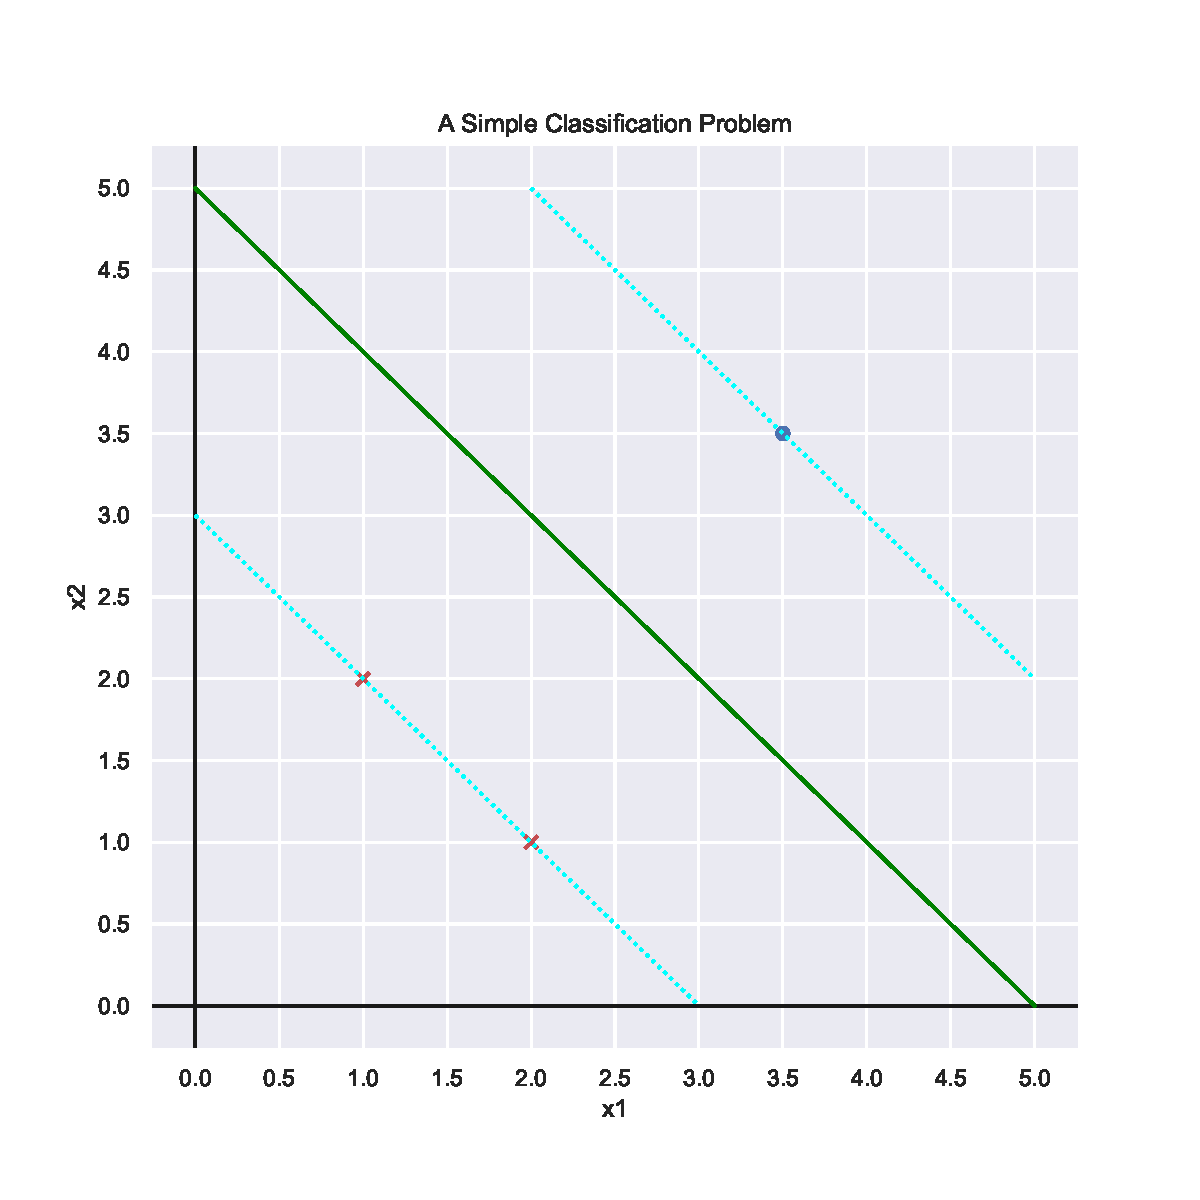
\epsfig{file=Figures/largest-margin.pdf, scale=0.6}
\caption{Three points to separate.}
\label{fig:largest-margin.pdf}
\end{figure}

Figure \ref{fig:largest-margin.pdf} on page \pageref{fig:largest-margin.pdf} shows three points that belong to
two different classes.  The blue dot at position $(3.5, 3.5)$ belongs to class $1$, while the two red crosses
at position $(1,2)$ and $(2,1)$ belong to the class $-1$.  When we build a classifier to separate these two
classes, we would ideally like the decision boundary to be the green line that passes through the points $(0,5)$ and
$(5,0)$, since this line has the biggest distance from both classes.  Figure
\ref{fig:largest-margin-logistic.pdf} on page \pageref{fig:largest-margin-logistic.pdf} shows how logistic regression
deals with with this problem.

\begin{figure}[!th]
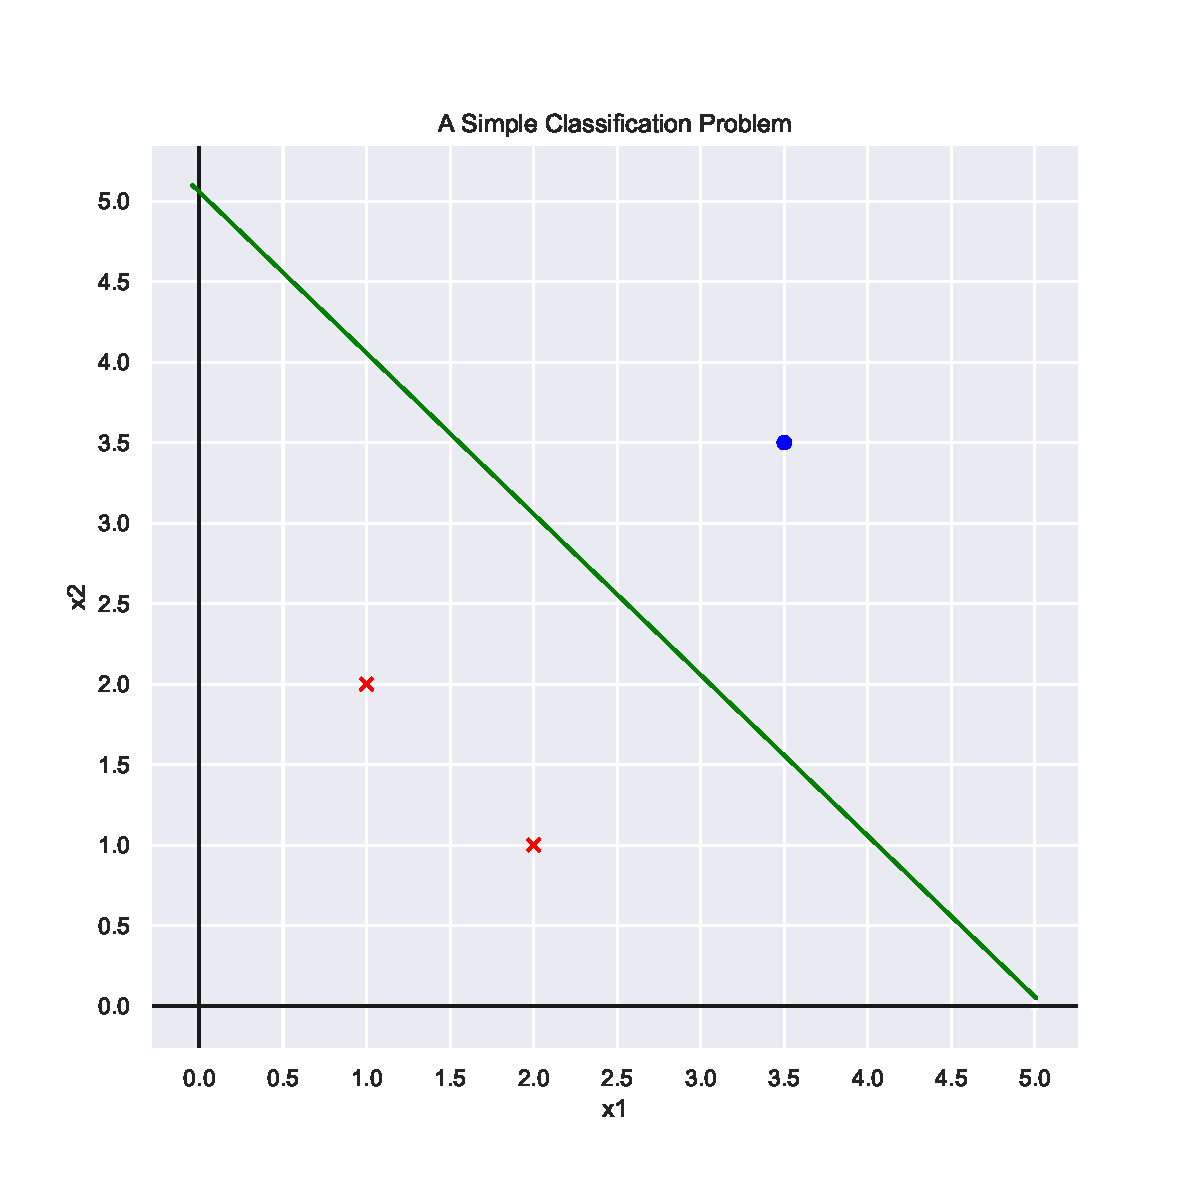
\epsfig{file=Figures/largest-margin-logistic.pdf, scale=0.6}
\caption{Three points separated by logistic regression.}
\label{fig:largest-margin-logistic.pdf}
\end{figure}

A close inspection of Figure \ref{fig:largest-margin-logistic.pdf} shows that the decision boundary calculated
by logistic regression is nearer to the blue dot than it is to the red crosses.  If we add a large number of
blue points right next to the first blue points, the decision boundary found by logistic regression moves away
from the blue points, as shown in Figure \ref{fig:largest-margin-more.pdf} on
page \pageref{fig:largest-margin-more.pdf},
then the decision boundary moves away from the first blue point that marks the margin of the two classes.
These new blue points do not add real information, since they are further away from the red crosses than the
first blue point.  Hence it is counter-intuitive that the addition of these points changes the decision boundary.

\begin{figure}[!th]
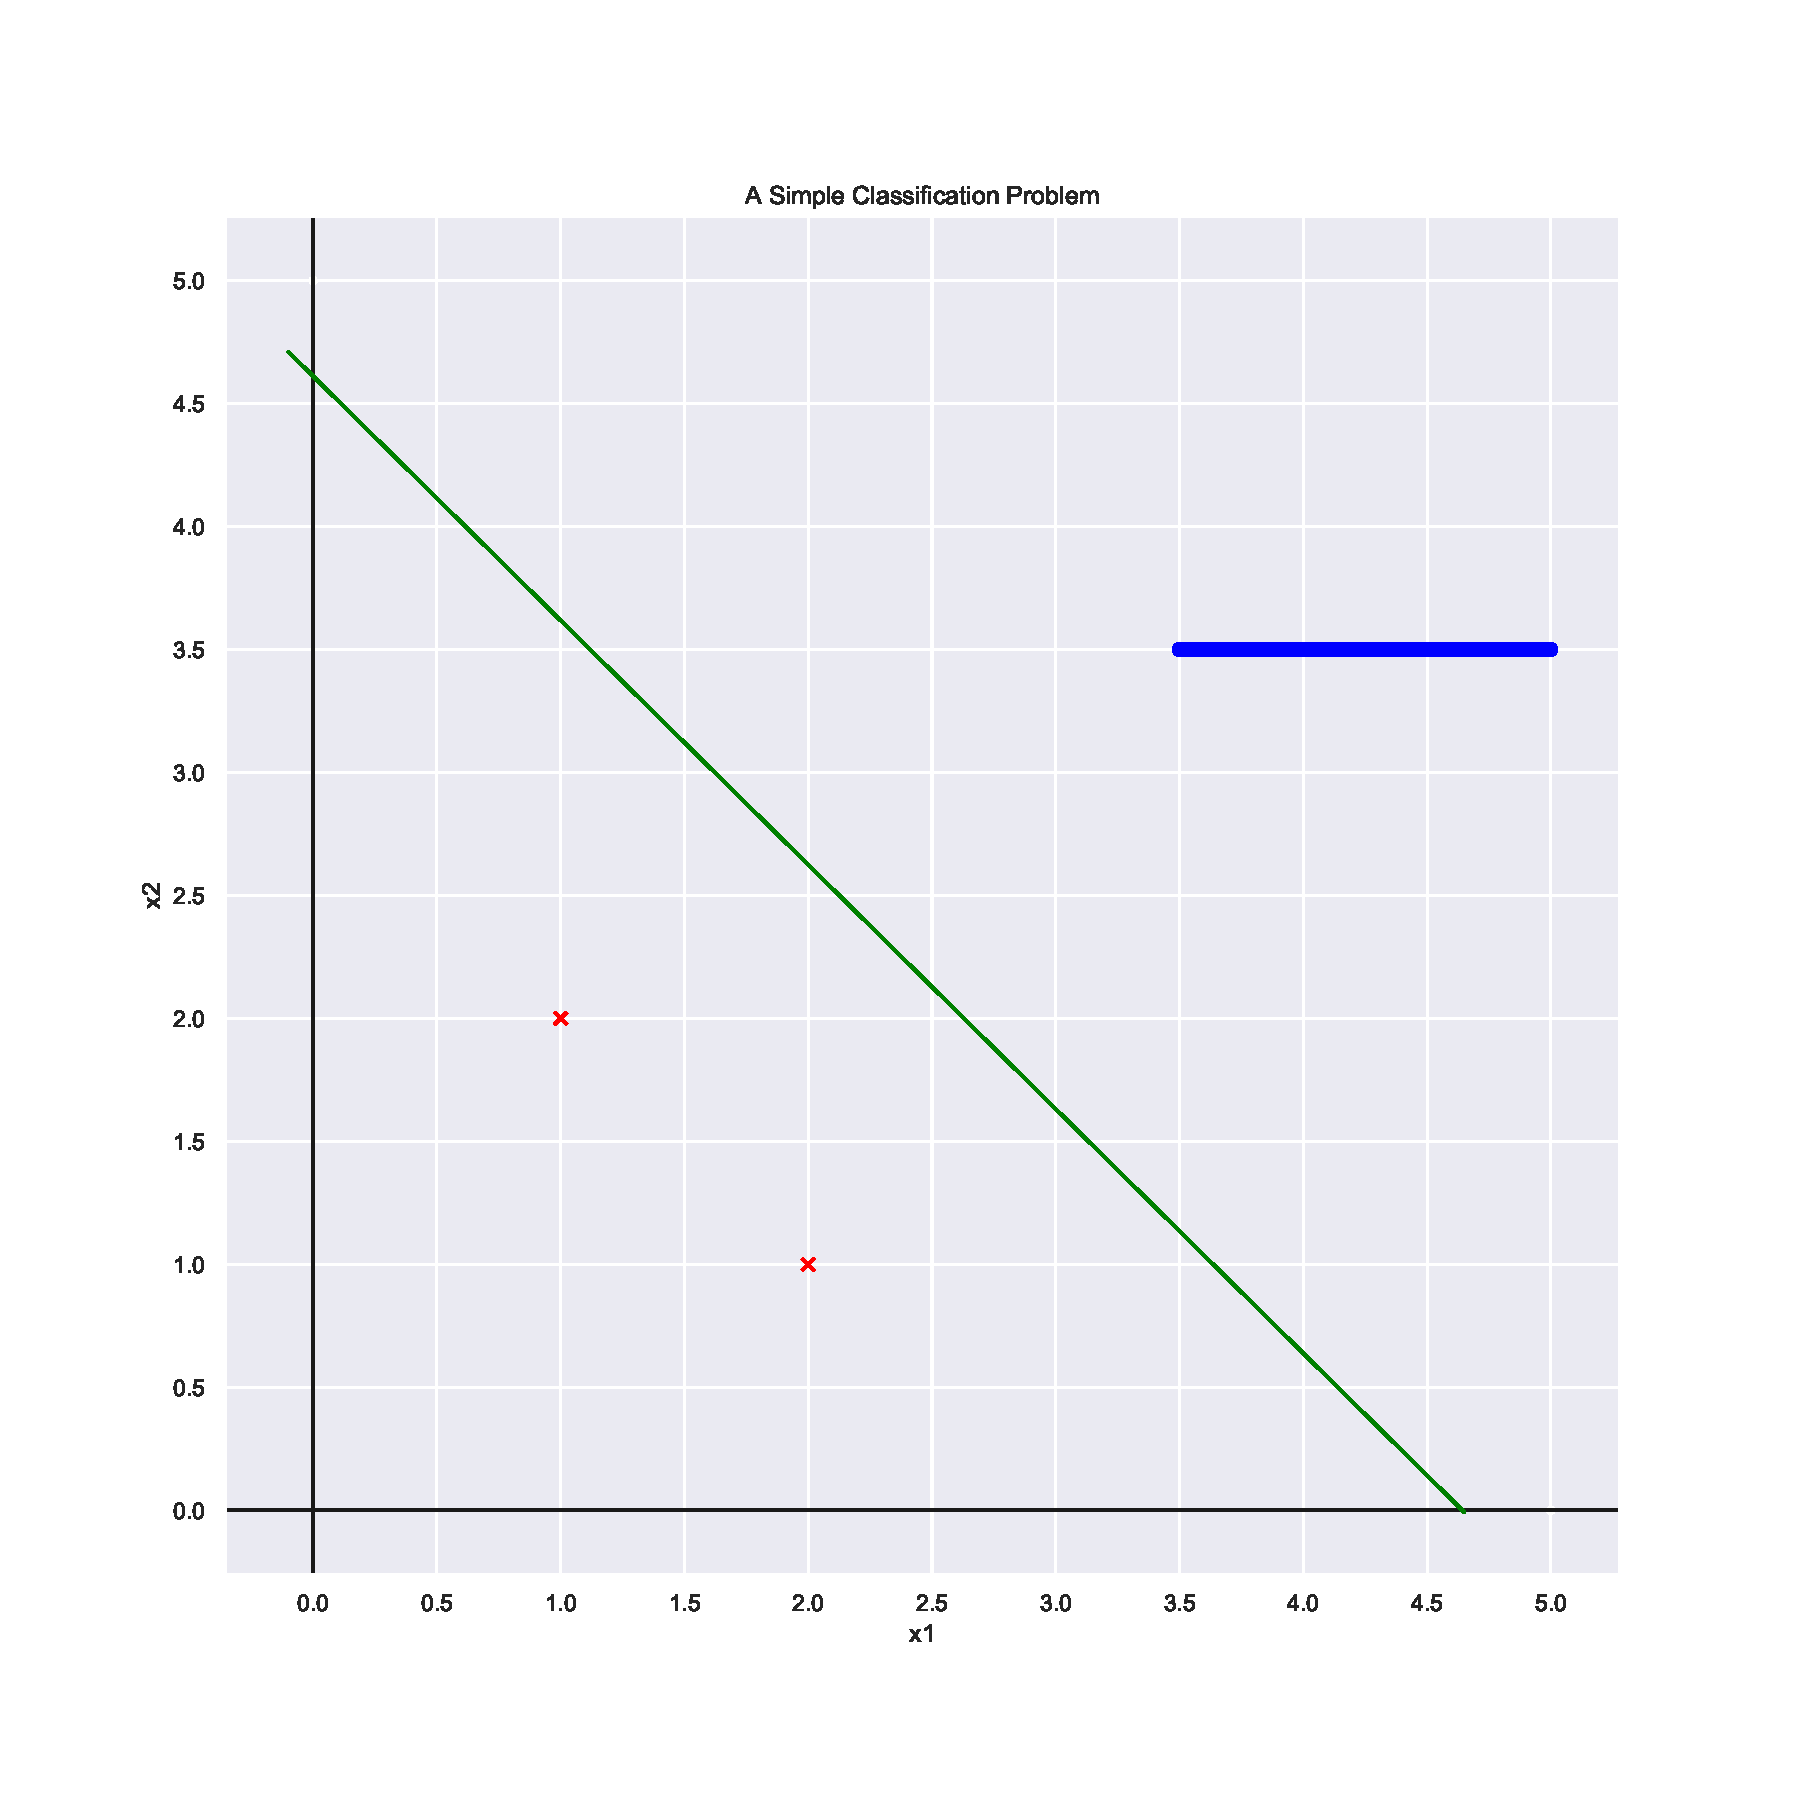
\epsfig{file=Figures/largest-margin-more.pdf, scale=0.5}
\caption{Points separated by logistic regression.}
\label{fig:largest-margin-more.pdf}
\end{figure}

\subsection{The Mathematical Theory of Support Vector Machines}
The main idea of support vector machines is to have a decision boundary that is \blue{as simple as possible} and that
\blue{separates the different classes as much as possible}.  In two dimensions, the simplest decision boundary is a
line.  In $n$ dimensions, the simplest decision boundary is an $(n-1)$-dimensional hyperplane.
A hyperplane separates two different classes as much as possible if the distance to both classes is maximized.

A hyperplane can be defined by a vector $\mathbf{w}$ that is perpendicular to the hyperplane together with a
bias $b$:  A vector $\mathbf{x}$ is an element of the hyperplane if and only if
\\[0.2cm]
\hspace*{1.3cm}
$\mathbf{w} \cdot \mathbf{x} + b = 0$.
\\[0.2cm]
In order for the decision boundary to separate the positive examples from the negative examples, we add the
following two conditions.  If $\mathbf{x}^{(i)}$ is a positive example, then we don't just want that 
\\[0.2cm]
\hspace*{1.3cm}
$\mathbf{w} \cdot \mathbf{x}^{(i)} + b \geq 0$.
\\[0.2cm]
Instead, we demand that 
\begin{equation}
  \label{eq:svm-1}
  \mathbf{w} \cdot \mathbf{x}^{(i)} + b \geq 1
\end{equation}
holds.  Similarly, if $\mathbf{x}^{(i)}$ is a negative example, we want to have that
\begin{equation}
  \label{eq:svm-2}
    \mathbf{w} \cdot \mathbf{x}^{(i)} + b \leq -1
\end{equation}
holds.  Let us define the class of a positive example to be $+1$ and the
class of a negative example to be $-1$.  Let $y_i$ denotes the class of example $\mathbf{x}^{(i)}$.
Let us multiply equation \ref{eq:svm-1} by $y_i = 1$.  Unsurprisingly, we get
\begin{equation}
  \label{eq:svm-3}
  y_i \cdot \bigl(\mathbf{w} \cdot \mathbf{x}^{(i)} + b) \geq 1.
\end{equation}
Similarly, let us multiply equation \ref{eq:svm-1} by $y_i = -1$.  This time, things get more interesting
as the direction of the inequality is flipped:
\begin{equation}
  \label{eq:svm-4}
    y_i \cdot \bigl(\mathbf{w} \cdot \mathbf{x}^{(i)} + b) \geq 1.
\end{equation}
Notice that the equations \ref{eq:svm-3} and \ref{eq:svm-4} are the same!  Hence
inequation \ref{eq:svm-3} holds for both positive and negative examples.  We rewrite the last inequation as
\begin{equation}
  \label{eq:svm-5}
    y_i \cdot \bigl(\mathbf{w} \cdot \mathbf{x}^{(i)} + b\bigr) - 1 \geq 0.
\end{equation}
Those vectors $\mathbf{x}^{(i)}$ that satisfy the equality
\\[0.2cm]
\hspace*{1.3cm}
$y_i \cdot \bigl(\mathbf{w} \cdot \mathbf{x}^{(i)} + b\bigr) - 1 = 0$
\\[0.2cm]
are at the \blue{margins} of their respective classes and are called \blue{support vectors}.  These vectors
have the smallest distance to the hyperplane defined by $\mathbf{w}$ and $b$.  Let us compute the width of the
separation of the positive class from the negative class if the decision boundary is given by the  equation
$\mathbf{w} \cdot \mathbf{x} + b = 0$.  To this end, assume that $\mathbf{x}_+$ is a positive support vector,
i.e.~we have
\begin{equation}
  \label{eq:svm-6}
  \mathbf{w} \cdot \mathbf{x}_+ + b = 1,  
\end{equation}
while $\mathbf{x}_-$ is a negative support vector and therefore satisfies
\begin{equation}
  \label{eq:svm-7}
  \mathbf{w} \cdot \mathbf{x}_- + b = -1.  
\end{equation}
Since the vector $\mathbf{w}$ is perpendicular to the hyperplane that defines the decision boundary, the $\mathtt{width}$
between the positive and the negative example is given by the projection $\mathbf{x}_+ - \mathbf{x}_-$ on the normalized vector $\mathbf{w}$:
\begin{equation}
  \label{eq:svm-8}
 \mathtt{width} = \bigl(\mathbf{x}_+ - \mathbf{x}_-\bigr) \cdot \frac{\mathbf{w}}{||\mathbf{w}||} =
\bigl(\mathbf{x}_+ \cdot \mathbf{w} - \mathbf{x}_-\cdot \mathbf{w}\bigr) \cdot \frac{1}{||\mathbf{w}||}   
\end{equation}
If we subtract equation \ref{eq:svm-7} from equation \ref{eq:svm-6}, the constant $b$ cancels and we are left
with 
\\[0.2cm]
\hspace*{1.3cm}
$\mathbf{x}_+ \cdot \mathbf{w} - \mathbf{x}_- \cdot \mathbf{w} = 2$.  
\\[0.2cm]
Substituting this equation into equation \ref{eq:svm-8} yields the equation
\\[0.2cm]
\hspace*{1.3cm}
$\ds \mathtt{width} = \frac{2}{||\mathbf{w}||}$.
\\[0.2cm]
Hence in order to maximize the width of the separation of the two classes from the decision boundary we have to
minimize the size of the vector $\textbf{w}$ subject to the constraints given in equation \ref{eq:svm-5}.  Now minimizing $\mathbf{w}$
is the same as minimizing
\\[0.2cm]
\hspace*{1.3cm}
$\ds \frac{1}{2} \cdot ||\mathbf{w}||^2 = \frac{1}{2} \cdot \sum\limits_{k=1}^d w_k^2$,
\\[0.2cm]
where $d$ is the number of features.
Determining a minimum of a function that is subject to a set of constraints requires us to use 
\href{https://en.wikipedia.org/wiki/Lagrange_multiplier}{Lagrange multipliers}.  Assuming our training set 
has the form $\{ \mathbf{x}^{(1)}, \cdots \mathbf{x}^{(n)} \}$,
we define the \blue{Lagrangian} $\mathcal{L}(\mathbf{w}, b, \alpha_1, \cdots, \alpha_n)$ as follows:
\\[0.2cm]
\hspace*{1.3cm}
$\ds \mathcal{L}(\mathbf{w}, b, \alpha_1, \cdots, \alpha_n) := 
 \frac{1}{2} \cdot ||\mathbf{w}||^2 - 
\sum\limits_{i=1}^n \alpha_i \cdot \bigl(y_i \cdot(\mathbf{w} \cdot \mathbf{x}_i + b) - 1\bigr).
$ 
\\[0.2cm]
The sum in this Lagrangian sums over all training examples although not all training examples have to satisfy
the constraint
\\[0.2cm]
\hspace*{1.3cm}
$y_i \cdot(\mathbf{w} \cdot \mathbf{x}_i + b) - 1 = 0$.
\\[0.2cm]
This is not a problem because for those $i \in \{1,\cdots,\}$ where we only have the inequality
\\[0.2cm]
\hspace*{1.3cm}
$y_i \cdot(\mathbf{w} \cdot \mathbf{x}_i + b) - 1 \geq 0$
\\[0.2cm]
we can just assume that the corresponding Lagrange multiplier $\alpha_i$ is  equal to $0$.
A necessary condition for the values of $\mathbf{w}$, $b$ and $\alpha_i$ that minimize $\mathcal{L}$ is that
the partial derivatives of $\mathcal{L}$ with respect to $w_k$, $b$ and $\alpha_i$ are all $0$.  Let us first compute the partial derivative of $\mathcal{L}$
with respect to $w_k$:
\\[0.2cm]
\hspace*{1.3cm}
$\ds \frac{\partial \mathcal{L}}{\partial w_k} = 
 w_k - \sum\limits_{i=1}^n \alpha_i \cdot y_i \cdot x^{(i)}_k = 0
$
\\[0.2cm]
Therefore, we must have that
\\[0.2cm]
\hspace*{1.3cm}
$w_k = \sum\limits_{i=1}^n \alpha_i \cdot y_i \cdot x^{(i)}_k $ 
\\[0.2cm]
and this implies
\begin{equation}
  \label{eq:svm-9}
  \mathbf{w} = \sum\limits_{i=1}^n \alpha_i \cdot y_i \cdot \mathbf{x}^{(i)}
\end{equation}
Therefore the vector $\mathbf{w}$ is a linear combination of the \blue{support vectors}, where a vector
$\mathbf{x}^{(i)}$ is a support vector iff  $\alpha_i \not= 0$.  Hence a support vector $\mathbf{x}^{(i)}$ 
must satisfy the equality
\\[0.2cm]
\hspace*{1.3cm}
$y_i \cdot(\mathbf{w} \cdot \mathbf{x}_i + b) - 1 = 0$.
\\[0.2cm]
Next, let us compute the partial derivative of $\mathcal{L}$ with respect to $b$. We have
\\[0.2cm]
\hspace*{1.3cm}
$\ds \frac{\partial \mathcal{L}}{\partial b} = - \sum\limits_{i=1}^n \alpha_i \cdot y_i = 0$
\\[0.2cm]
which implies that
\begin{equation}
  \label{eq:svm-10}
  \sum\limits_{i=1}^n \alpha_i \cdot y_i = 0  
\end{equation}
Let us rewrite the Lagrangian by substituting $\mathbf{w}$ with the right hand side of equation \ref{eq:svm-9}:
\\[0.2cm]
\hspace*{0.3cm}
$
\begin{array}[t]{lcl}
  \mathcal{L} & = &
                    \ds \frac{1}{2} \cdot \left(\sum\limits_{i=1}^n \alpha_i \cdot y_i \cdot \mathbf{x}^{(i)}\right)
                    \cdot \left(\sum\limits_{j=1}^n \alpha_j \cdot y_j \cdot \mathbf{x}^{(j)}\right) 
               - \sum\limits_{i=1}^n \alpha_i \cdot \left( y_i \cdot\left( \mathbf{x}^{(i)} \cdot
                    \left(\sum\limits_{j=1}^n \alpha_j \cdot y_j \cdot \mathbf{x}^{(j)} \right) + b\right) -1 \right) \\[0.6cm]
              & = &
                    \ds \frac{1}{2} \cdot \sum\limits_{i=1}^n \sum\limits_{j=1}^n \alpha_i \cdot \alpha_j \cdot
                    y_i \cdot y_j \cdot \bigl(\mathbf{x}^{(i)} \cdot \mathbf{x}^{(j)}\bigr) 
                    - \sum\limits_{i=1}^n \sum\limits_{j=1}^n \alpha_i \cdot \alpha_j \cdot y_i \cdot y_j \cdot
                     \bigl( \mathbf{x}^{(i)} \cdot \mathbf{x}^{(j)} \bigr) - b \cdot\underbrace{\sum\limits_{i=1}^n \alpha_i \cdot y_i}_{=0}
                    + \sum\limits_{i=1}^n \alpha_i \\[0.6cm]
              & = & \ds \sum\limits_{i=1}^n \alpha_i - \frac{1}{2} \cdot \sum\limits_{i=1}^n
                    \sum\limits_{j=1}^n \alpha_i \cdot \alpha_j \cdot y_i \cdot y_j \cdot
                    \bigl(\mathbf{x}^{(i)} \cdot \mathbf{x}^{(j)}\bigr)
\end{array}
$
\\[0.2cm]
Now, the \blue{crucial observation} is the following:  The Lagrangian $\mathcal{L}$ only depends on the dot
products $\mathbf{x}^{(i)} \cdot \mathbf{x}^{(j)}$.  Why is this a big deal?  Often, a set of data point is not
linearly separable in the given space.  However, it might be possible to transform the feature vectors
$\mathbf{x} \in \mathbb{R}^d$ into some higher dimensional space $\mathbb{R}^h$ where $h > d$ and the tow
classes are separable.  Concretely, it is sometimes possible to define a transformation function
\\[0.2cm]
\hspace*{1.3cm}
$\Phi: \mathbb{R}^d \rightarrow \mathbb{R}^h$
\\[0.2cm]
such that the set of transformed data points
$\bigl\{\Phi(\mathbf{x}^{(1)}), \cdots, \Phi(\mathbf{x}^{(n)})\bigr\}$ is linearly separable.
The question then is to find such a transformation $\Phi$.  Here is the punch line:  As the Lagrangian does
only depend on dot products, it is sufficient to define the transformed dot products
\\[0.2cm]
\hspace*{1.3cm}
$\Phi\bigl(\mathbf{x}\bigr) \cdot \Phi\bigl(\mathbf{y}\bigr) $.
\\[0.2cm]
This is done with the help of so called \blue{kernel functions}:  We define the dot product
$\Phi\bigl(\mathbf{x}\bigr) \cdot \Phi\bigl(\mathbf{y}\bigr)$ as
\\[0.2cm]
\hspace*{1.3cm}
$\Phi\bigl(\mathbf{x}\bigr) \cdot \Phi\bigl(\mathbf{y}\bigr) := k(\mathbf{x}, \mathbf{y})$
\\[0.2cm]
where $k$ is called a \blue{kernel function}.  There are two kernel functions that are quite popular:
\begin{enumerate}
\item \blue{Polynomial kernels} have the form
      \\[0.2cm]
      \hspace*{1.3cm}
      $k(\mathbf{x}, \mathbf{y}) = (\mathbf{x} \cdot \mathbf{y} + c)^n$,
      \\[0.2cm]
      where $n$ is a natural number called the \blue{degree} of the kernel.
      The number $c$ is a hyperparameter that is often set to $1$.
\item \blue{Gaussian kernels} have the form
      \\[0.2cm]
      \hspace*{1.3cm}
      $\ds k(\mathbf{x}, \mathbf{y}) = \exp\left( \frac{||\mathbf{x}-\mathbf{y}||^2}{2 \cdot \sigma^2}\right)$.
      \\[0.2cm]
      Here, $\sigma$ is a hyperparameter.  
\end{enumerate}
Using a kernel function to simulate a parameter transformation is known as the \blue{kernel trick}.    
Experience has shown that the kernel functions given above often enable us to transform a data set into a space where the
data set is linearly separable.  Figure \ref{fig:strange-data.pdf} on page \pageref{fig:strange-data.pdf} shows
a set of point that is separable using a support vector machine with a Gaussian kernel.

\begin{figure}[!th]
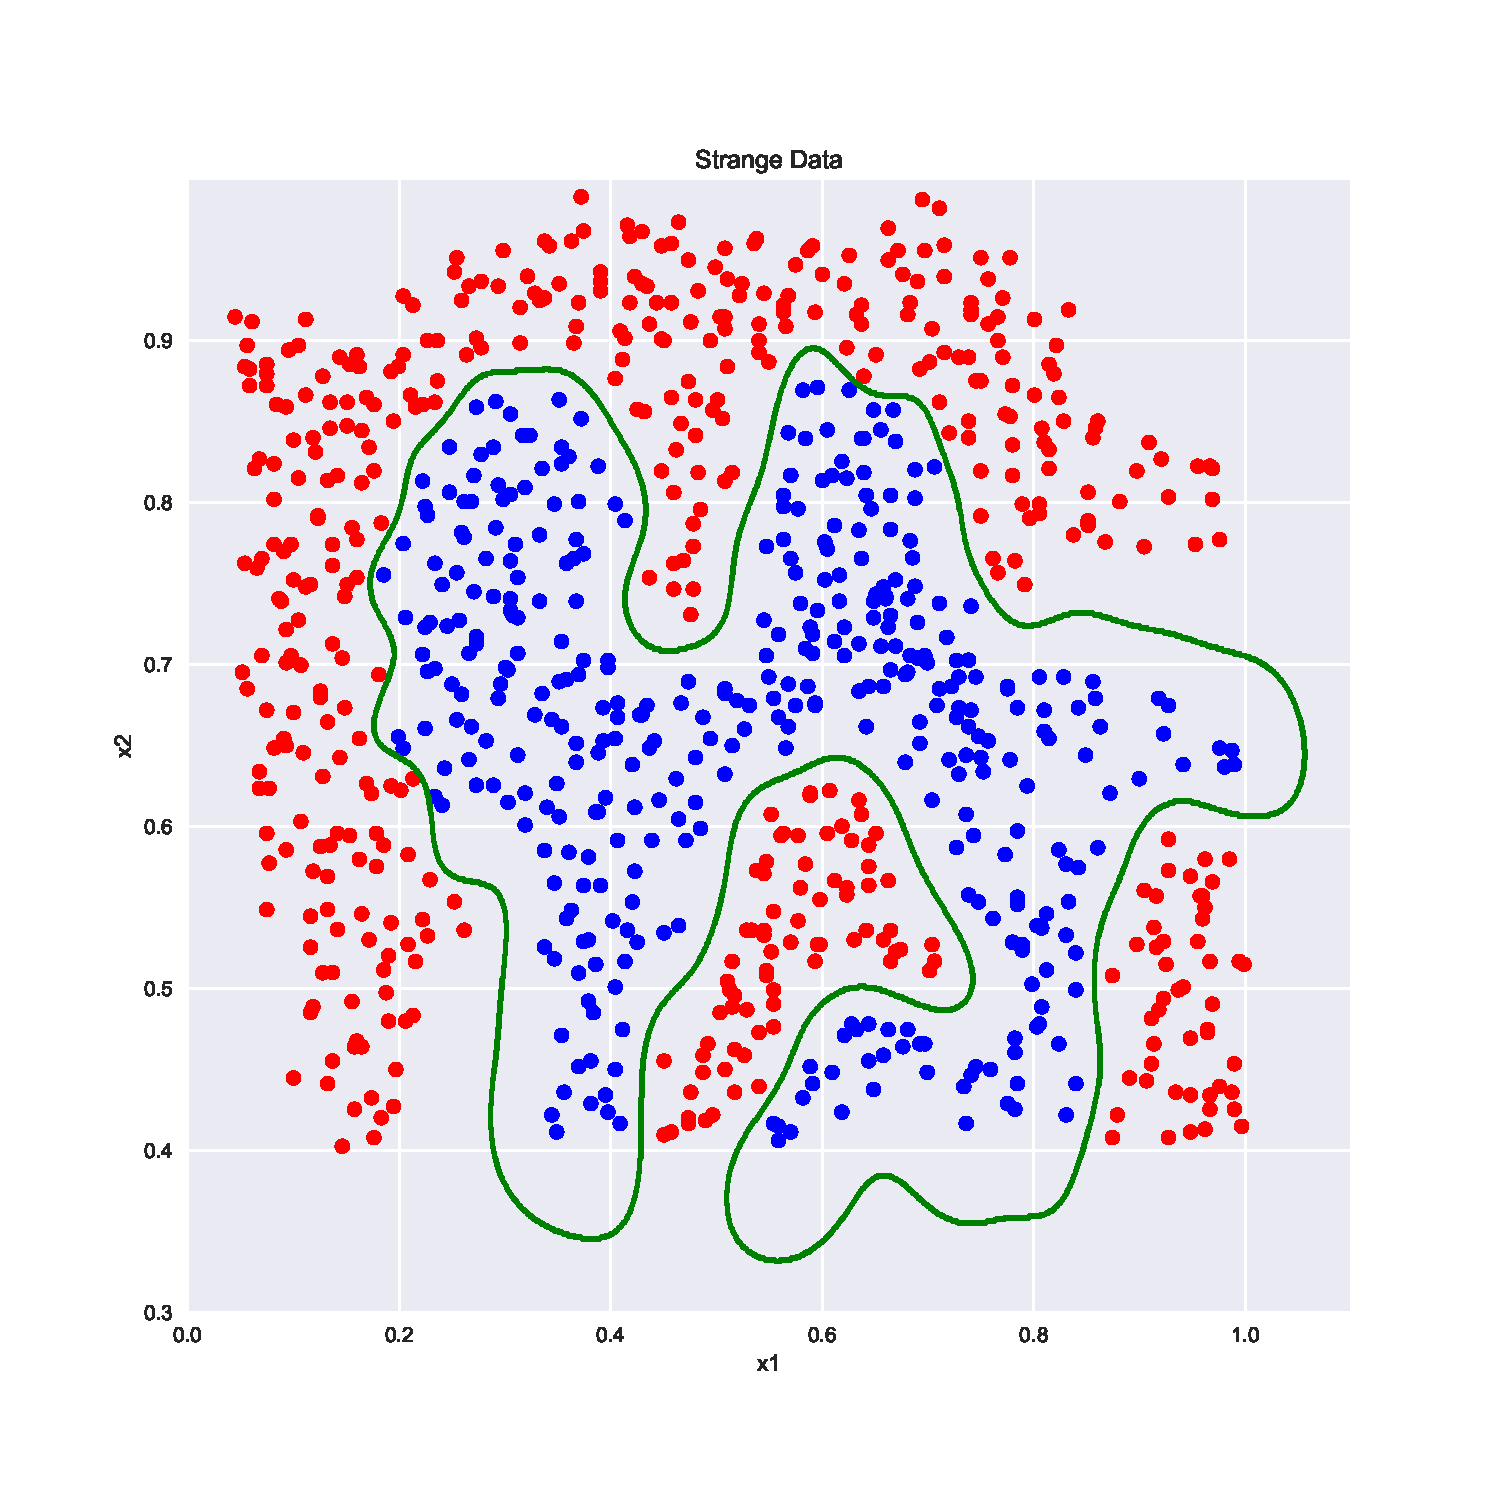
\epsfig{file=Figures/strange-data.pdf, scale=0.6}
\caption{Points separated by a support vector machine.}
\label{fig:strange-data.pdf}
\end{figure}

If you want to know more about support vector machines, the free book
\href{https://www.syncfusion.com/ebooks/support_vector_machines_succinctly}{Support Vector Machines Succinctly}
by Alexandre Kowalczyk \cite{kowalczyk:2017} is a good place to start.


%%% Local Variables:
%%% mode: latex
%%% TeX-master: "artificial-intelligence"
%%% End:
 
